\documentclass[11pt,a4paper]{article}
\usepackage[margin=24mm,headheight=15pt]{geometry}
\usepackage[T1]{fontenc}
\usepackage[utf8]{inputenc}
\usepackage{lmodern,microtype,amsmath,amssymb,graphicx,booktabs,longtable,array,tabularx}
\usepackage{float,caption,enumitem,xcolor,fancyhdr,listings,tikz}
\usetikzlibrary{arrows.meta,positioning,fit,backgrounds}
\usepackage[hyphens]{url}
\usepackage[colorlinks=true,linkcolor=blue!45!black,citecolor=blue!45!black,urlcolor=blue!55!black,bookmarksnumbered=true]{hyperref}
\definecolor{navy}{HTML}{15384C}
\definecolor{teal}{HTML}{206B7D}
\definecolor{orange}{HTML}{B76A16}
\hypersetup{pdftitle={CARE-ECG: Detailed Methodology, Experimental Protocols, and Evidence-Based Results},pdfauthor={CARE-ECG repository technical documentation},pdfsubject={Independent implementation and retrospective experimental audit}}
\pagestyle{fancy}\fancyhf{}
\fancyhead[L]{\small\textcolor{navy}{CARE-ECG: methodology and experimental evidence}}
\fancyhead[R]{\small 28 October 2026}
\fancyfoot[L]{\footnotesize Independent implementation; research use}
\fancyfoot[R]{\thepage}
\setlength{\parindent}{0pt}\setlength{\parskip}{5.5pt}
\setlist[itemize]{leftmargin=18pt,itemsep=2pt,topsep=3pt}
\setlist[enumerate]{leftmargin=21pt,itemsep=3pt,topsep=3pt}
\renewcommand{\arraystretch}{1.16}
\captionsetup{font=small,labelfont=bf,skip=7pt}
\lstset{basicstyle=\ttfamily\footnotesize,breaklines=true,columns=fullflexible,keepspaces=true,frame=single,rulecolor=\color{black!15},backgroundcolor=\color{black!2},showstringspaces=false}
\newcommand{\code}[1]{\texttt{\detokenize{#1}}}
\newcommand{\scope}[1]{\par\smallskip\noindent\fcolorbox{teal!35}{teal!4}{\parbox{\dimexpr\linewidth-2\fboxsep-2\fboxrule}{#1}}\par\smallskip}
\newcommand{\fig}[3]{\begin{figure}[htbp]\centering\includegraphics[width=#2\linewidth]{figures/#1.pdf}\caption{#3}\label{fig:#1}\end{figure}}
\newcommand{\gt}{\mathrm{GT}}
\newcommand{\norm}[1]{\left\lVert #1\right\rVert}
\begin{document}
\hypersetup{pageanchor=false}
\begin{titlepage}
\vspace*{12mm}
{\Large\color{teal} RESEARCH IMPLEMENTATION TECHNICAL REPORT\par}
\vspace{13mm}
{\Huge\bfseries\color{navy} CARE-ECG\par}
\vspace{5mm}
{\LARGE\bfseries Detailed Methodology,\par Experimental Protocols,\par and Evidence-Based Results\par}
\vspace{11mm}
{\large Waveform representation learning, Bayesian reasoning,\par counterfactual search, evidence-grounded reporting,\par full-dataset ingestion, adaptive attacks, and DPO co-evolution\par}
\vspace{13mm}
{\large Code and evidence review: 28 October 2026\par}
\vspace{6mm}
\href{https://github.com/elakhatibi/CARE-ECG-Full-Datasets}{github.com/elakhatibi/CARE-ECG-Full-Datasets}
\vfill
\scope{\textbf{Report identity.} This manuscript describes the independent implementation in the repository and audits saved local experiments. It is separate from the original CARE-ECG publication. Measured outcomes, retrospective analyses, implemented but unevaluated capabilities, and pending dataset work are identified separately. No new training or clinical study was conducted to prepare this document.}
\vspace{5mm}
{\small The report contains aggregate results only. Patient identifiers, waveforms, credentials, and model weights are not embedded. Numerical tables and figures are regenerated from the accompanying \code{build_evidence.py}; the input hashes and aggregate analysis are archived in \code{evidence.json}.}
\end{titlepage}
\hypersetup{pageanchor=true}
\pagenumbering{roman}

\section*{Abstract}
\addcontentsline{toc}{section}{Abstract}
CARE-ECG couples ECG representation learning with probabilistic reasoning, retrieval, and traceable report generation. This report specifies the implemented pipeline in sufficient detail to distinguish its computations from the stronger causal and clinical interpretations that the available evidence cannot establish. A supervised temporal variational autoencoder uses an InceptionTime-style encoder to learn 64 latent coordinates from 12-lead, 100~Hz, 10-second ECGs. Training-only quantiles discretize posterior means; an ordered K2 search with a BDeu score fits a categorical Bayesian network. Exact inference, local posterior sensitivity, and single-coordinate evidence edits support explanation. A separate, validation-locked multinomial stack over three legacy benchmark-derived probability sources supplies the released diagnosis. History, Diagnosis, Causal-RAG, and Response agents construct fact-tagged reports with lexical verification and fallback.

The completed supervised study uses 17,084 eligible PTB-XL training ECGs, 2,146 validation ECGs, and all 2,158 eligible fold-10 ECGs from 1,877 patients. Reanalysis of the saved released predictions gives accuracy 76.83\%, macro precision 68.87\%, macro recall 67.74\%, and macro F1 68.25\%. A retrospective 10,000-resample patient-cluster bootstrap gives a macro-F1 interval of 65.45--70.90\%. HYP is the weakest class, with recall 40.58\% and F1 42.11\%. A subsequent waveform-specialist search improves validation F1 but reduces fold-10 F1 and is not promoted. Report checks show perfect lexical evidence coverage while passing all 500 wrong diagnoses, illustrating their limited diagnostic scope.

A separate locked waveform-callable security study evaluates four attacks, two constraints, two complete-system query budgets, and three seeds on ten selected clean-correct patients per split. Its held-out cell-average targeted attack success is 25.0\% at both budgets; untargeted success rises from 52.5\% to 56.7\%. These are automated, nonclinical outcomes for the internal model, excluding the cached diagnostic stack. The clinical incorrect-release endpoint is not evaluable. Full acquisition and indexing are complete for PTB-XL~1.0.1 (21,837 ECGs) and 43,670 released Expert-ECG-QA source rows; MIMIC-IV-ECG acquisition remains pending at the snapshot. No completed MIMIC faithfulness or full QA benchmark score is claimed. Differences in artifacts, label projection, generation, and evaluation keep the original-paper reproduction status \textbf{NOT REPRODUCED}.

A later nine-attack, 19-patient validation comparison gives adaptive v2 K2/K3 26.32\% amplitude-constrained exact-target success, compared with PGD at 21.05\%, with spectral ties and mixed untargeted outcomes. Two finite-action policies are then trained with patient-balanced, frozen-reference DPO in a bounded attacker--verifier loop. In two small real-data rounds, attacker and verifier training losses decrease, but no candidate passes validation promotion; exported incumbents remain the priors. These are development checks, not evidence of full-cohort, held-out, or clinical DPO improvement.

\textbf{Keywords:} ECG; variational autoencoder; InceptionTime; Bayesian network; causal attribution; retrieval-augmented generation; patient-grouped evaluation; adversarial robustness; direct preference optimization; co-evolution; reproducibility.

\clearpage
\tableofcontents
\clearpage
\pagenumbering{arabic}

\section{Scope, evidence, and research questions}
\label{sec:scope}
\subsection{What system is being described?}
The original CARE-ECG article proposes a physiological reasoning stream and an agentic report stream for explainable, counterfactual ECG interpretation~\cite{care}. The repository implements an independent engineering realization of those modules. The locally documented experiment does not have the original trained checkpoints, clinical graph priors, licensed knowledge collection, exact split files, prompts, or evaluator implementation. Its replacements are part of the method and must remain visible when interpreting results.

There are three distinct execution settings. \textbf{Released fixed-candidate classification} uses saved, record-aligned external expert probabilities to determine diagnosis while an internal InceptionTime model supplies explanatory context. \textbf{Waveform-callable inference} recomputes the internal model from the waveform and can process new ECGs; it does not manufacture external scores for unseen records. \textbf{Security evaluation} perturbs raw-mV waveforms and attacks this callable internal model. The cached external stack is excluded because it cannot respond to waveform edits. Accuracy of the released stack and robustness of the internal victim therefore refer to different diagnostic mechanisms.

\subsection{Research questions and available evidence}
The report addresses six questions:
\begin{enumerate}
\item How are waveforms converted into latent variables, categorical evidence, diagnostic probabilities, retrieved facts, and reports?
\item Under the declared PTB-XL single-label projection, what performance does the frozen released system achieve, and which classes account for its errors?
\item Do validation improvements survive fixed-candidate evaluation, and what uncertainty remains after accounting for repeated ECGs per patient?
\item What does a small locked adversarial study establish about the waveform-callable victim, and what clinical-security conclusions remain unmeasured?
\item How are adaptive v2 attacks and the two DPO controllers implemented, and do their saved development runs demonstrate validation improvement?
\item How does full-corpus support relate to completed evaluation, particularly for different PTB-XL versions, MIMIC-IV-ECG, and released QA tasks?
\end{enumerate}

Four evidence classes are used consistently: \emph{saved measurements} from experiment JSON/JSONL files; \emph{new retrospective analyses} of those frozen outputs; \emph{implemented capabilities} verified in source code; and \emph{uncompleted studies} for which no outcome is supplied. The accompanying scripts do not update models, choose thresholds for deployment, or relabel records. The original paper's numbers are reference targets, not observations from this repository.

\subsection{Snapshot and traceability}
The earlier published source commit is:\par
{\small\code{e98a5b0a2735f69a49c31e6fca2e624880376809}}\par
 The classification and specialist experiments were recorded on 21 October 2026; the expanded locked security study on 26 October 2026. The report's aggregate reanalysis and data-status review are dated 28 October 2026, America/Los\_Angeles. Archived security logs bind their own historical code identities; later full-corpus and momentum changes must not be retroactively attributed to those locked runs. Adaptive v2 and two-role DPO development runs were recorded on 28 October 2026. These local extensions and this report are not asserted to be included in the published source commit. The report records current source hashes separately from historical experiment identities.

\begin{table}[htbp]\centering\small
\begin{tabularx}{\linewidth}{p{0.28\linewidth}Xp{0.25\linewidth}}
\toprule Experiment & Statistical coverage & Interpretation \\\midrule
Released classification & 2,158 eligible fold-10 ECGs; 1,877 patients & Fixed-candidate evaluation; prior test knowledge disclosed.\\
Historical security & Ten clean-correct patients per split; four attacks; three seeds & Locked automated internal-victim outcomes.\\
Adaptive v2 & All 19 clean-correct patients in a 30-patient validation pool; nine attacks & Development comparison; one seed, one-query budget.\\
DPO co-evolution & Six training and six disjoint validation patients; two rounds & Optimization and audit demonstrated; no promotion.\\
Full source ingestion & Complete PTB-XL 1.0.1 and released QA indexes; MIMIC pending & Acquisition coverage; no invented benchmark score.\\\bottomrule
\end{tabularx}
\caption{Evidence map. Patient caps and endpoint differences are part of each study, even though uncapped ingestion and security workflows are implemented.}
\label{tab:evidencemap}\end{table}

\section{Datasets, task definition, and patient coverage}
\label{sec:data}
\subsection{PTB-XL: supervised task versus full database}
PTB-XL provides 12-lead ECGs, SCP-ECG annotations, and recommended patient-separated folds~\cite{ptbxl,ptbxl_data}. The completed local supervised experiment uses the 21,799-row release described in its run metadata as version~1.0.3. There are 18,869 identifiable patients in the full local index. The acquisition module conservatively leaves this older local directory's version unverified when no acquisition receipt exists; this provenance limitation does not change the saved prediction cohort or hashes.

The supervised task is a \emph{single-label projection} to the ordered set
\begin{equation}
\mathcal{Y}=\{\mathrm{NORM},\mathrm{MI},\mathrm{STTC},\mathrm{CD},\mathrm{HYP}\}.
\end{equation}
These abbreviations denote normal ECG, myocardial infarction, ST/T changes, conduction disturbance, and hypertrophy, respectively. For each eligible superclass, the preparation code retains SCP likelihoods and selects the superclass with the highest eligible likelihood. Ties use the displayed order. This changes a potentially multi-label annotation problem into a categorical one; performance is consequently conditional on this projection and is not an official multi-label PTB-XL benchmark result.

Exactly 411 local records have no eligible diagnostic superclass. They are excluded from supervised labels, leaving 21,388 eligible ECGs, but are retained in the all-record index. No missing annotation is converted to NORM. The training set uses folds~1--8; fold~9 supplies validation; fold~10 supplies fixed-candidate evaluation. Table~\ref{tab:cohorts} is independently counted from the prepared NPZ archives, including unique patients.

\begin{table}[htbp]\centering\small
\begin{tabular}{lrrrrrrr}
\toprule
Split & ECGs & Patients & NORM & MI & STTC & CD & HYP \\
\midrule
Train & 17084 & 14823 & 7386 & 3406 & 3408 & 2380 & 504 \\
Validation & 2146 & 1917 & 928 & 407 & 426 & 310 & 75 \\
Test & 2158 & 1877 & 932 & 418 & 421 & 318 & 69 \\
\bottomrule
\end{tabular}

\caption{Prepared supervised cohorts. Counts are ECGs unless explicitly labeled patients. No patient or record overlaps between these three splits were found.}
\label{tab:cohorts}\end{table}

Raw split sizes are 17,418, 2,183, and 2,198; excluded counts are 334, 37, and 40, respectively. Thus ``complete fold-10 coverage'' in the classifier study means all 2,158 \emph{eligible} ECGs, not all 2,198 raw fold-10 records. In the test cohort NORM accounts for 43.19\% of records and HYP for only 3.20\%. Macro metrics prevent the largest class from dominating the reported result, although the small HYP support still limits precision of class-specific conclusions.

\subsection{Paper-count PTB-XL acquisition}
The paper lists 21,837 ECGs from 18,885 patients. The acquisition configuration chooses PTB-XL~1.0.1 because its published count agrees with that number~\cite{ptbxl_old}. This is an explicit version choice; a count match is not proof of the authors' exact dataset revision. At the report snapshot, download, extraction, publisher-checksum verification, and indexing of this release are complete: all 21,837 records are indexed and no requested waveform is missing.

The downloaded release contains 100~Hz and 500~Hz waveforms. It is kept in a separate directory and index from the local completed experiment. The previously trained model, labels, stack arrays, and fold-10 measurements are not silently replaced. Older and newer PTB-XL releases share many ECGs and must not be pooled as independent external validation data. Full-corpus inference over either release includes training records unless a fold filter is supplied; it cannot be called held-out evaluation merely because every patient is processed.

\subsection{MIMIC-IV-ECG}
The open waveform release MIMIC-IV-ECG~1.0 contains approximately 800,000 diagnostic ECGs from nearly 160,000 patients~\cite{mimic}. The implementation downloads its versioned archive, verifies publisher checksums after extraction, and streams metadata into a disk-backed JSONL index. At the report snapshot MIMIC remains the sole pending acquisition item. A partial archive is not counted as a completed or evaluated dataset.

The paper uses this resource primarily for retrieval faithfulness rather than treating its ECGs as a ready-made five-class QA test. The saved local classifier has a five-superclass output space fitted to PTB-XL. Its MIMIC outputs would therefore be transferred model predictions, not newly established categorical ground truth. Waveform availability also does not imply that the paper's report corpus, case linkage, or faithfulness adjudication has been reconstructed. This report supplies no completed MIMIC classification, grounding, or faithfulness score.

\subsection{Expert-ECG-QA source normalization}
The QA source is pinned to revision \code{4fcb46974eed422532772caa483a5e621f006ff1} of the dataset publisher's repository~\cite{qa_repo,qa}. All 43,670 released source rows in 11 JSON task files are indexed; 17,024 patient identifiers can be identified in that source. The original CARE-ECG paper lists 47,211 QA pairs covering 12 tasks. Released source rows and semantic QA turns are different units, and some rows contain nested dialogues or multiple questions. The difference of 3,541 between these two headline counts does not establish exactly 3,541 missing independent questions. The implementation preserves the available payloads and documents the discrepancy instead of inventing examples.

\begin{table}[htbp]\centering\small
\begin{tabular}{p{0.78\linewidth}r}
\toprule
Released source task & Rows \\
\midrule
Cardiology Knowledge (Basic Knowledge Q\&A) & 2592 \\
Complex diagnosis (analysis of difficult diseases) & 1931 \\
Cross modal diagnosis (ECG Text corresponding diagnosis) & 20032 \\
ECG Knowledge (Basic Q\&A) & 2247 \\
Generate risk assessment & 2931 \\
Long text diagnosis & 2931 \\
Medical entity extraction & 2623 \\
Medical inquiry, multiple rounds of dialogue between doctors and patients & 2931 \\
Memory correction & 2931 \\
Patient prognosis (prognostic analysis) & 1164 \\
Patient's right to know & 1357 \\
\bottomrule
\end{tabular}

\caption{Complete released QA source-row inventory for the pinned revision. These are acquisition counts, not successfully answered or scored questions.}
\label{tab:qa}\end{table}

The cross-modal file reverses the usual field roles: its A field contains the query and Q field the reference answer. The normalizer handles this explicitly. Questions in nested structures are extracted without appending reference answers to the prompt. Unknown patient identifiers remain unknown. Every output retains the source task and reference separately for later task-specific adjudication.

Where a QA study ID links to a MIMIC waveform, a temporary SQLite lookup joins that study and checks the patient ID before inference. Rows without a valid waveform link take an explicitly labeled text-only path using source context and retrieval. This avoids fabricating ECG features for text-only cases. The available runner is an inference and audit tool; it does not reproduce the missing publisher evaluation procedure or a complete multi-turn conversational benchmark. The existing two-row QA smoke output is integration evidence only.

\subsection{Acquisition integrity and memory behavior}
The downloader uses resumable \code{.zip.part} files, verifies valid HTTP range responses, and resumes from the actual received offset. Retry limits apply to consecutive failures without progress, allowing very long downloads to recover from intermittent interruptions. Exclusive locks protect dataset acquisition and manifest updates. Extraction rejects traversal and symlink entries and uses archive CRC checks; PhysioNet SHA-256 manifests are subsequently checked. Index manifests include source, requested and verified version, hashes, row and patient counts, waveform availability, pending datasets, and errors.

Waveform inference reads a bounded batch instead of loading the entire database. If batch size is $b$, lead count $C$, and resampled length $T$, waveform working memory grows as $O(bCT)$ rather than $O(NCT)$. QA joins use disk-backed lookup. Source arrays for the historical diagnostic stack are a separate record-aligned artifact contract and cannot be generalized by row position to another database.

\section{End-to-end system architecture}
\label{sec:architecture}
Figure~\ref{fig:architecture} separates the shared explanatory path from the released external diagnosis path. There is no training step in which a free-form LLM output becomes the supervised label for the completed categorical experiment. The agent names denote software components with explicit inputs and outputs; the default execution does not instantiate a collection of independently trained autonomous LLMs.

\begin{figure}[htbp]\centering
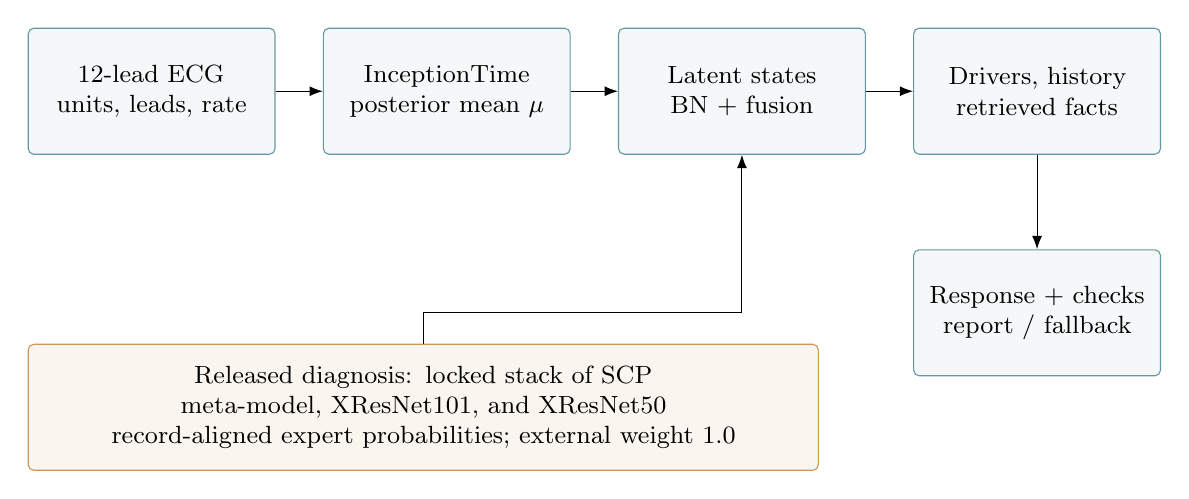
\begin{tikzpicture}[node distance=5mm and 6mm,>=Latex,
 box/.style={draw=teal!70,rounded corners=2pt,fill=teal!5,align=center,font=\small,text width=29mm,minimum height=16mm},
 wide/.style={box,text width=98mm,fill=orange!7,draw=orange!70}]
\node[box] (x) {12-lead ECG\\units, leads, rate};
\node[box,right=of x] (enc) {InceptionTime\\posterior mean $\mu$};
\node[box,right=of enc] (bn) {Latent states\\BN + fusion};
\node[box,right=of bn] (rag) {Drivers, history\\retrieved facts};
\node[box,below=12mm of rag] (report) {Response + checks\\report / fallback};
\node[wide,below=12mm of x,anchor=west] (stack) at (x.west |- report.west) {Released diagnosis: locked stack of SCP meta-model, XResNet101, and XResNet50\\record-aligned expert probabilities; external weight 1.0};
\draw[->] (x)--(enc);\draw[->] (enc)--(bn);\draw[->] (bn)--(rag);\draw[->] (rag)--(report);
\draw[->] (stack.north) -- ++(0,4mm) -| (bn.south);
\end{tikzpicture}
\caption{Computational paths. The orange box supplies the released diagnostic posterior; the teal path supplies internal representations and explanatory evidence. Security and new-record full-corpus inference use the waveform-callable internal model without the orange record-keyed source.}
\label{fig:architecture}\end{figure}

\subsection{Waveform and metadata contracts}
The generic NPZ interface accepts finite signals with aligned labels, record IDs, patient IDs, timestamps, and folds where available. A standard model input is $x\in\mathbb{R}^{12\times1000}$. The full-corpus WFDB loader requires exactly the standard leads and reorders them to I, II, III, aVR, aVL, aVF, V1--V6. It uses physical units from each header: V is multiplied by 1,000; microvolts by 0.001; mV is unchanged. Unsupported units or incompatible lead sets raise an error.

Nonfinite samples are interpolated within each lead; an entirely nonfinite lead becomes zeros. If resampling is required, the code uses polyphase resampling with the source-to-target integer ratio reduced by its greatest common divisor. Longer signals are center-cropped and shorter signals symmetrically zero-padded to the configured duration. These repair and padding rules are deterministic. The completed experiment uses 100~Hz rather than the original paper's 500~Hz input description, which is a documented architectural deviation.

\subsection{Training-only global standardization}
Preparation for the completed study leaves per-record normalization disabled. A scalar mean and standard deviation are fitted over training-fold records, leads, and samples:
\begin{equation}
\bar{x}=\frac{1}{NCT}\sum_{n,c,t}x_{nct},\qquad
s=\sqrt{\frac{1}{NCT}\sum_{n,c,t}(x_{nct}-\bar{x})^2},\qquad
x'=(x-\bar{x})/s.
\end{equation}
The stored values are $\bar{x}=-0.0008252534$~mV and $s=0.2322225810$~mV. Validation and inference reuse these constants. Global scaling preserves relative amplitudes between leads and records, unlike independently standardizing every trace. Optional robust and z-score per-record policies exist for other configurations but are not the policy behind the reported completed study. Security constraints apply to raw mV before this model normalization.

\section{Representation learning and optimization}
\label{sec:representation}
\subsection{Temporal encoder and classifier}
The completed model uses a six-module InceptionTime-style backbone inspired by multiscale time-series convolutions~\cite{inception}. A stem maps 12 leads to 48 channels with a kernel of length 15 and stride 2, followed by a 48-to-96 convolution of kernel 9 and stride 2. Group normalization and SiLU follow these convolutions. The resulting temporal length is 250 for the 1,000-sample input.

Each Inception module has a 96-to-24 bottleneck, three 24-channel convolution branches with kernel lengths 15, 7, and 3, and a max-pooling branch followed by a 96-to-24 pointwise convolution. Concatenation recovers 96 channels, followed by batch normalization, ReLU, and channel dropout of 0.1. Residual shortcuts span every three modules. A learned scalar attention score $a_t$ pools temporal features $h_t$:
\begin{equation}
\alpha_t=\frac{\exp(a_t)}{\sum_{u}\exp(a_u)},\qquad h=\sum_t\alpha_t h_t\in\mathbb{R}^{96}.
\end{equation}
Separate linear heads produce a 64-dimensional posterior mean and log variance. Log variance is clamped to $[-12,12]$. The supervised classifier consumes the pooled encoder feature $h$, not the sampled latent vector: layer normalization, a 96-to-192 linear layer, SiLU, dropout, and a 192-to-5 output layer. This bypass matters: class discrimination can improve without proving that every latent coordinate is an interpretable clinical biomarker.

\subsection{Variational objective and deterministic inference}
The approximate posterior and reparameterization are
\begin{equation}
q_\phi(z\mid x)=\mathcal{N}(\mu_\phi(x),\operatorname{diag}(\sigma^2_\phi(x))),\qquad
z=\mu+\sigma\odot\epsilon,\quad\epsilon\sim\mathcal{N}(0,I).
\end{equation}
The decoder projects $z$ to a $96\times20$ seed, applies three transposed convolutions with stride 4 and widths 128, 64, and 32, then a 12-lead output convolution. Linear interpolation aligns the reconstruction to the requested length when necessary. The implementation minimizes
\begin{align}
\mathcal{L}_{\mathrm{rec}}&=\frac{1}{bCT}\sum_{n,c,t}(\hat{x}_{nct}-x'_{nct})^2,\\
\mathcal{L}_{\mathrm{KL}}&=-\frac{1}{2bd}\sum_{n,j}\left(1+\log\sigma^2_{nj}-\mu_{nj}^2-\sigma^2_{nj}\right),\\
\mathcal{L}&=\mathcal{L}_{\mathrm{rec}}+\beta_e\mathcal{L}_{\mathrm{KL}}+2\mathcal{L}_{\mathrm{CE}},
\qquad\beta_e=0.0005\min(1,e/10).
\end{align}
Cross-entropy uses balanced class weights and label smoothing 0.03. The KL term is averaged across dimensions, so its effective scale differs from a summed per-record KL. During training, samples are stochastic; downstream fitting and inference use $z=\mu$ with the model in evaluation mode. The code can encode and classify without decoding at inference.

The class name \code{CausalVAE} follows the repository and original architectural proposal. A standard-normal factorized prior and a downstream learned DAG do not, by themselves, identify causal variables. In contrast to a fully identified structural causal representation, the implementation has no supervised mapping from $z_j$ to QTc, ST elevation, or another measured physiological variable. Latents remain anonymous coordinates.

\subsection{Optimization and augmentation}
AdamW uses learning rate 0.001 and weight decay $10^{-4}$; batch size is 64. Gradients are clipped to norm 1.0. A cosine schedule decays toward $10^{-5}$ over the configured 40 epochs. Early stopping monitors validation macro F1, using patience 8 and minimum change $10^{-4}$; best weights are restored. The saved run completed 20 epochs and selected epoch 12. The seed is 42 and the saved configuration specifies CPU execution; elapsed training time and peak training memory were not archived, so throughput claims are omitted.

Each record is selected for augmentation with probability 0.5. Active records may receive multiplicative scaling within $\pm5\%$, Gaussian noise with standard deviation 0.01 times the clean lead standard deviation, sinusoidal baseline wander scaled by 0.02 of that deviation, a zero-filled temporal shift up to 1\% of length, and independent lead dropout probability 0.01. At least one lead is retained. Augmented inputs are reconstructed against the clean normalized target, yielding a denoising training task. The configuration labels these perturbations as mild; no independent clinical preservation study is implied by that description.

\begin{table}[htbp]\centering\small
\begin{tabular}{lr@{\qquad}lr}\toprule
Parameter & Value & Parameter & Value\\\midrule
Leads / rate / duration & 12 / 100 Hz / 10 s & Latent dimension & 64\\
Encoder width / modules & 96 / 6 & Classifier hidden width & 192\\
Inception kernels & 15, 7, 3 & Dropout & 0.1\\
Maximum epochs / batch & 40 / 64 & Selected / completed epoch & 12 / 20\\
Learning rate / decay & 0.001 / cosine & Weight decay & 0.0001\\
Maximum KL weight & 0.0005 & Warm-up epochs & 10\\
Classification weight & 2.0 & Label smoothing & 0.03\\
Gradient norm limit & 1.0 & Early-stop patience & 8\\\bottomrule
\end{tabular}
\caption{Saved internal waveform-model configuration. These values describe the experiment, not recovered original-paper hyperparameters.}\label{tab:hyperparameters}\end{table}

\section{Discrete Bayesian reasoning and explanation}
\label{sec:bayes}
\subsection{Quantile states and ordered graph search}
For each latent coordinate, the discretizer fits thresholds at training-only quantiles 0.2, 0.4, 0.6, and 0.8. An inference value is assigned by right-sided insertion into these four thresholds, producing states 0--4. Thresholds and feature order are serialized. All 64 latent coordinates have training variance above the saved active-unit threshold $10^{-4}$, but nonzero variance is not evidence of disentanglement or clinical meaning.

The network variables are ordered $z_0,\ldots,z_{63},y$. Greedy K2 adds only predecessors as parents, which guarantees an acyclic graph and places diagnosis last. Required prior edges are allowed if they respect the order and parent cap. In this completed study the PTB-XL ontology has no clinician-reviewed causal edges, so the learned dependencies arise from the training data and imposed ordering. Each node has at most five parents. Search uses the Bayesian Dirichlet equivalent uniform score with equivalent sample size $\eta=5$:
\begin{equation}
S_i=\sum_{j=1}^{q_i}\left[\log\Gamma(\eta/q_i)-\log\Gamma(\eta/q_i+N_{ij})+
\sum_{k=1}^{r_i}\left(\log\Gamma(\eta/(q_ir_i)+N_{ijk})-\log\Gamma(\eta/(q_ir_i))\right)\right].
\end{equation}
Here $r_i$ is node cardinality, $q_i$ is the number of parent configurations, and $N_{ijk}$ counts training observations. Starting from required edges, the learner repeatedly adds the admissible parent with greatest score improvement until no improvement exceeds $10^{-9}$ or the parent cap is reached. This is an order-constrained greedy search, not a global DAG optimum.

Categorical conditional tables are then estimated with per-cell additive smoothing $\alpha=1$:
\begin{equation}
\widehat{P}(v_i=k\mid\mathrm{Pa}_i=j)=\frac{N_{ijk}+\alpha}{N_{ij}+r_i\alpha},\qquad
P(v_1,\ldots,v_m)=\prod_i P(v_i\mid\mathrm{Pa}_i).
\end{equation}
The smoothing convention for final CPTs is separate from the BDeu search prior. Conditioning observed factors, multiplying tables, and summing out hidden variables implement exact variable elimination for $P(y\mid\tilde z)$.

\subsection{Fusion and attribution scope}
The general internal pipeline allows a validation-selected mixture
\begin{equation}
p_{\mathrm{int}}=(1-w_n)p_{\mathrm{BN}}+w_n p_{\mathrm{neural}},\qquad
p'_{c}=\operatorname{softmax}_c(\log p_{\mathrm{int},c}+b_c).
\end{equation}
The released artifact fixes $w_n=1$ and $b_c=0$. External-expert fusion first blends internal neural and external probabilities; the released diagnostic setting assigns external weight~1. Thus the final output probabilities equal the external stack probabilities, within floating-point precision. The Bayesian network still produces a separate explanatory posterior but has zero weight in the released diagnosis.

For a declared diagnosis class $c$, driver importance is the largest absolute change in the scoped posterior when one supported state is substituted:
\begin{equation}
I_j=\max_{s\in\mathcal{S}_j\setminus\{\tilde z_j\}}
\left|p_c(\tilde z)-p_c(\tilde z_{-j},s)\right|.
\end{equation}
The output also records the signed difference, best alternative state, and directed graph path. With all latents observed and diagnosis last, only direct parents of diagnosis affect its conditional posterior, so the implementation avoids testing irrelevant fully observed ancestors. Where neural/external weight removes all fused sensitivity, the agent explicitly switches to \code{bayesian_component} scope. It does not assert that changing those coordinates changes the external expert's decision.

\subsection{Single-factor counterfactual search}
For a requested target $y^*$, the engine enumerates supported alternative states of candidate diagnosis parents while holding all other evidence fixed. It returns an achieving edit if
\begin{equation}
\arg\max_c P(c\mid \tilde z_{-j},s)=y^*.
\end{equation}
Among achieving candidates it prefers smaller ordinal state movement, then larger target posterior, with deterministic feature/state tie breaking. If no edit changes the winner but some improve the target probability, it returns the best improvement with \code{found=false}. If the target already wins it returns a zero-edit result. The output's edit distance is the number of changed factors (zero or one), whereas ordinal movement is used to rank alternative states.

The worst-case number of edited posterior evaluations is at most $|\mathrm{Pa}(y)|(K-1)$ for $K$ states, excluding the baseline; with a five-parent cap and five bins it is at most 20. The counterfactual belongs to the explicitly selected posterior scope. It is an observational evidence-edit search, not a validated intervention $P(y\mid\operatorname{do}(z_j=s))$, and it does not produce an actionable physical ECG or patient treatment.

\section{Agent coordination, retrieval, and reporting}
\label{sec:agents}
\subsection{History and Diagnosis agents}
The History Agent receives the current latent vector and an optional set of dated reference encodings. If matching patient records exist, it chooses the latest timestamp; otherwise it chooses the nearest latent reference by Euclidean distance and marks the mode as surrogate. With no history the mode is none. It reports the full latent difference and three largest shifts. Callers are responsible for supplying genuinely prior records: choosing the maximum timestamp alone does not establish that the record preceded the current ECG. Surrogate similarity cannot be interpreted as longitudinal change in that patient.

The Diagnosis Agent computes Bayesian and fused probabilities, chooses the highest-probability label, obtains scoped drivers and paths, and optionally requests a counterfactual. The released outputs contain three ranked Bayesian-component drivers per record. The report backbone therefore exposes its own reasoning evidence, while also declaring the separation from the external diagnosis posterior.

\subsection{Diagnosis-aware causal RAG}
RAG combines retrieval from an explicit corpus with generation~\cite{rag}. Here the completed artifact uses the lightweight TF-IDF implementation rather than the optional sentence-transformer backend. It indexes unigrams and adjacent bigrams with smoothed IDF,
\begin{equation}
\operatorname{idf}(t)=\log\frac{1+D}{1+\operatorname{df}(t)}+1,
\end{equation}
log-scaled term counts, and $L_2$ normalization. The query is enriched with the original question, named latent states, and the three leading diagnostic hypotheses. Document scores combine cosine similarity and diagnosis metadata:
\begin{equation}
s(d,q)=0.8\langle v_d,v_q\rangle+0.2\,s_{\mathrm{metadata}}(d,p).
\end{equation}
Documents explicitly tagged with competing diagnostic classes are excluded unless they also match the selected diagnosis. Generic evidence remains eligible. The top five eligible facts with score at least $10^{-8}$ are returned, with source ID, document ID, lexical and structured scores, and matching metadata.

The saved PTB-XL knowledge graph contains 50 ontology nodes and 49 taxonomy edges. These links support retrieval and provenance and are explicitly marked as noncausal. They are not clinician-reviewed physiological priors. The bundled demonstration collection is also not a comprehensive clinical guideline corpus. Even a perfectly cited response may be limited by the underlying corpus or by diagnosis-conditioned exclusion of conflicting evidence; a future evaluation should test confirmation bias and evidence recall directly.

\subsection{Response construction and alternative generators}
The Response Agent assembles fields for the question, temporal context, predicted label, posterior, driver states, attribution scope, requested counterfactual, and numbered retrieved facts. It instructs the generator to preserve the supplied diagnosis, cite each factual claim, and avoid unobserved waveform findings. The deterministic template is the generator behind the reported completed classification run. It makes output replayable but does not measure open-ended LLM reasoning quality.

Optional local Hugging Face and API-backed generators are implemented. Their checkpoint/model, decoding settings, access, knowledge corpus, and privacy eligibility would need to be fixed for a new experiment. The configurable model string in the saved YAML is not proof that that API model was called: the saved backend is \code{template}. No reported result here is attributed to a newly run LLaMA or API experiment.

\subsection{Verification, fallback, and abstention}
The first check measures how many retrieved facts are reflected in the report:
\begin{equation}
\mathrm{HR}=1-\frac{1}{|R|}\sum_{r\in R}\mathbb{1}[\operatorname{match}(r,e)],
\end{equation}
with HR~1 for no facts. Matching combines 0.7 token containment and 0.3 sorted-token sequence similarity, taking the best sentence match and thresholding at 0.32. This is primarily retrieved-fact recall, despite the name hallucination risk. Repeating every supplied fact can yield HR~0 even with a wrong diagnosis or an added false assertion.

The complementary unsupported-claim rate segments the report, ignores specified nonclinical prefixes, parses fact citations, and checks lexical support for each remaining sentence against its cited facts. It is a support proxy, not entailment or medical truth. The response is flagged when HR exceeds 0.5 or unsupported-claim rate exceeds zero. With fallback enabled, a second draft omits the causal factors. If that still fails, an evidence-only rendering is produced and the abstention state is recorded. Audit outputs retain both drafts, scores, fallback use, and abstention. No verifier can establish that the model-predicted diagnosis is correct simply because its associated facts are repeated faithfully.

\section{Locked diagnostic stack and model selection}
\label{sec:stack}
\subsection{External probability sources and alignment}
The final classifier uses three replacement sources derived from the legacy PTB-XL benchmark repository~\cite{benchmark}. They are not recovered author checkpoints from CARE-ECG. The sources are (i) an SCP-aware HistGradientBoosting meta-model, (ii) official XResNet1D-101 exp0 SCP outputs collapsed to the five-class contract, and (iii) a legacy XResNet1D-50 checkpoint adapter. Each table includes probability rows, exact record IDs, and label order. Missing or repeated record IDs, nonfinite values, negative entries, incompatible labels, or misaligned rows are rejected. Legacy pickle-bearing arrays and serialized estimators are authenticated by SHA-256 before loading.

For the superclass adapter, scores of SCP codes mapping to each superclass are summed and the resulting five scores normalized. These are derived scores; they are not a learned categorical diagnosis head from the original paper. The SCP meta-model uses the original 71 code scores plus five aggregates per superclass: sum, maximum, mean, noisy-OR, and maximum logit. This yields 96 features. HistGradientBoosting uses 150 iterations, learning rate 0.07, at most 31 leaves, minimum leaf size 20, $L_2$ penalty~3, and square-root balanced sample weights, without internal early stopping.

\subsection{Multinomial stack objective and cross-fitting}
For three sources and five classes, the stack uses 15 concatenated log-probability features. Each feature is centered and scaled using the stack-fitting subset. The model is
\begin{equation}
u=[\log p^{(1)},\log p^{(2)},\log p^{(3)}],\quad
\bar u_j=(u_j-m_j)/(s_j+10^{-6}),\quad
p_{\mathrm{stack}}=\operatorname{softmax}(\bar uW+a).
\end{equation}
The optimizer minimizes weighted multinomial cross-entropy plus $\lambda\operatorname{mean}(W^2)$ with class weights $(N/(5n_c))^\rho$. It uses float64 LBFGS, at most 300 iterations, with zero-initialized weights and prevalence-initialized intercepts. The selected coefficient $\lambda=1.0$ is the direct penalty coefficient, not the inverse-C parameter used by some logistic-regression packages; $\rho=0.375$.

Five patient-grouped partitions of fold~9 produce stacker out-of-fold predictions. The base sources remain fixed; only the stacker is cross-fit. Hyperparameters maximize pooled OOF macro F1, breaking ties by accuracy. The same OOF values are used for selection and reporting, so they are selection estimates with optimism from reuse and base-expert validation history. They are not independent nested estimates of the complete workflow.

\subsection{Freeze, refit, and prior-test disclosure}
The selection lock froze source order, regularization, class weighting, and exact zero post-selection class offsets before inference for the current fold-10 candidate. After selection, the SCP meta-model was refit on folds~1--9. Its reported validation values still refer to the original folds-1--8 fit. This standard deployment refit changes the distribution supplied to a stack selected from earlier out-of-sample outputs, an additional source of validation-to-test shift.

The finalizer verifies artifact hashes, re-evaluates the stack from the aligned source tables, and saves provenance and zero offsets. The maximum discrepancy between final and supplied expert probabilities in the archived run is about $3.02\times10^{-8}$; the expert argmax is preserved. Prediction bookkeeping appends expected labels after model execution rather than supplying them to the decision method.

The lock also states that aggregate fold-10 performance from an earlier repository system was already known. Thus the current candidate was frozen before its evaluation, but fold~10 is not globally untouched. This report uses ``fixed-candidate fold-10 evaluation'' for that reason and avoids presenting the entire model-development process as a pristine first use of the test set.

% Remaining sections are included as a separate editable source file.
\section{Experimental design and statistical analysis}
\label{sec:experiments}
\subsection{Completed classification protocol}
The primary categorical outcome is macro F1 over the five fixed classes. Accuracy, macro precision, and macro recall are reported alongside it, without substituting one for another after observing the results. Base-model fitting uses the eligible training folds. Validation controls neural early stopping, internal mixture and bias selection, source screening, stacker settings, and specialist policy selection. Normalization, quantile thresholds, and the Bayesian network are fitted on the training set alone. The explicit official validation archive avoids the generic CLI's fallback record-level random holdout, which would require additional patient-group safeguards for longitudinal data.

The fixed-candidate run processes every eligible prepared fold-10 record with encoder batch size 64 and deterministic latent means. There are no saved prediction exceptions; all 2,158 unique record IDs are aligned exactly to the prepared split. Each report includes the model probabilities, selected diagnosis, continuous and categorical latent states, drivers, paths, facts, verifier scores, fallback and abstention status, and source provenance. The record-keyed external probabilities are supplied with expert weight 1.0. No current full-corpus download is used to enlarge or alter these historical evaluation labels.

For each class $c$, define true positives $TP_c$, false positives $FP_c$, and false negatives $FN_c$. The categorical measures are
\begin{align}
\mathrm{Acc}&=\frac{1}{N}\sum_i\mathbb{1}(\hat y_i=y_i),\\
P_{\mathrm{macro}}&=\frac{1}{5}\sum_c\frac{TP_c}{TP_c+FP_c},\qquad
R_{\mathrm{macro}}=\frac{1}{5}\sum_c\frac{TP_c}{TP_c+FN_c},\\
F1_{\mathrm{macro}}&=\frac{1}{5}\sum_c\frac{2P_cR_c}{P_c+R_c}.
\end{align}
Zero denominators contribute zero. Macro F1 is the mean of class F1 values; it is not generally the harmonic mean of macro precision and macro recall. All five classes occur in this test cohort. The report rebuilds the confusion matrix from saved predicted and expected labels and verifies that it recovers the archived aggregate values.

\subsection{Text-to-SCP protocol}
The mapper detects aliases and SCP codes, handles negation, and applies the declared fuzzy threshold 0.84. Its primary label is the first non-negated mapped mention. Mapping coverage and a separately labeled any-mention sensitivity measure are available. In the current deterministic reports, the supplied diagnosis is placed first and exactly one superclass is mapped per report. Therefore first-mention categorical accuracy, precision, recall, and F1 are identical to direct classification.

The permissive any-mention quantities are not alternative macro-classification metrics. They average per-report hit/precision/recall/F1 values using the set of mentioned codes. In this run there is one mapped code per report, so all four any-mention averages equal the hit rate 0.7683, whereas primary macro F1 remains 0.6825. A manuscript must not report 0.7683 as the primary five-class macro F1. This distinction matters even more when a free-form report lists multiple diagnoses.

\subsection{Retrospective patient-cluster bootstrap}
The report adds uncertainty to the frozen predictions, without retraining or selecting models. The 2,158 test ECGs belong to 1,877 distinct patients. For each of 10,000 bootstrap samples, 1,877 patients are sampled with replacement; all ECGs from each sampled patient are retained with the patient's multiplicity. A five-by-five confusion matrix is reconstructed and each metric recomputed. Percentile intervals use the 2.5th and 97.5th percentiles; the fixed analysis seed is 20261027.

This targets record-weighted performance while preserving within-patient dependence. It differs from independently resampling ECGs and from giving each patient equal weight in the point estimator. The same patient multiplicities are used for paired differences between systems. The analysis quantifies sampling uncertainty conditional on the fixed predictions. It excludes model refitting, hyperparameter-search uncertainty, original-paper protocol differences, prior test exposure, and external-site shift. All intervals are nominal pointwise intervals; no family-wise adjustment is made. They are a retrospective analysis of existing artifacts, not a preregistered confirmatory study.

\subsection{Confidence and report measures}
Confidence is the largest class probability. Log loss averages $-\log p_{i,y_i}$; the multiclass Brier score averages $\sum_c(p_{ic}-\mathbb{1}[y_i=c])^2$ without division by class count. ECE uses 15 equal-width confidence bins:
\begin{equation}
\mathrm{ECE}=\sum_b\frac{|B_b|}{N}\left|\mathrm{Acc}(B_b)-\overline p_{\max}(B_b)\right|.
\end{equation}
Selective risk sorts records by confidence and plots error among retained records. The 80\%-coverage result is a descriptive operating point on the test outputs, not a validated deployment threshold or evidence of safe abstention.

Local report measures are operational rather than clinical. CRC is the fraction of returned driver names mentioned in the text, with zero for no drivers. Groundedness is one minus unsupported-claim rate. Context relevance is lexical cosine between response and query; the local semantic-relevance proxy is lexical cosine between response and concatenated evidence. These use token-frequency vectors, not an independent semantic or clinical adjudicator. Attribution availability is reported for both the Bayesian component and the actual fused posterior. Finally, wrong-diagnosis pass rate asks how often the lexical gate passes a record whose categorical diagnosis is wrong.

\section{Classification, calibration, and report results}
\label{sec:results}
\subsection{Training dynamics and validation selection}
Figure~\ref{fig:training} shows the saved training and validation trajectories. The reported internal-model raw fold-9 macro F1 is 0.6511 at the selected epoch. Validation chooses neural mixture weight 1.0 over the Bayesian posterior, and later class-bias calibration raises this internal validation F1 to 0.6694. This calibration optimizes decision metrics on the same validation set; it is not a separately measured probability-calibration improvement. The final released stack uses zero post-selection class offsets rather than inheriting these internal calibration biases.

\fig{training}{1}{Saved waveform-model training trajectories. The dashed line marks restored epoch 12. Training uses augmentation and stochastic latent samples, whereas validation uses unaugmented inputs and posterior means. Reconstruction MSE is in globally standardized units.}

\begin{table}[htbp]\centering\small
\begin{tabular}{lrrrr}
\toprule
Neural weight & Accuracy (\%) & Macro P (\%) & Macro R (\%) & Macro F1 (\%) \\
\midrule
0.0 & 67.19 & 58.13 & 51.53 & 53.45 \\
0.25 & 70.13 & 64.93 & 55.21 & 57.62 \\
0.5 & 72.60 & 65.80 & 60.49 & 62.46 \\
0.75 & 73.72 & 65.24 & 64.11 & 64.53 \\
1.0 & 73.35 & 64.77 & 66.19 & 65.11 \\
\bottomrule
\end{tabular}

\caption{Internal Bayesian/neural fusion candidates on fold~9 before class-bias calibration. Selection is by macro F1. These are validation measurements, not independent ablations on an untouched test set.}\label{tab:fusion}\end{table}

Table~\ref{tab:fusion} makes a central architectural result explicit: the pure Bayesian component has validation macro F1 0.5345, and the best tested mixture places all diagnosis weight on the neural head. Adding the causal representation or graph therefore cannot be credited with the released classification improvement without a different controlled experiment. The saved graph has 65 variables and 179 edges, with three direct diagnosis parents, $z_{39}$, $z_{54}$, and $z_{55}$. The saved knowledge index has 54 documents. These counts establish the deployed artifact's structure, not causal identification or corpus adequacy.

The selected three-source stack reaches fold-9 accuracy 0.7628, macro precision 0.7040, macro recall 0.6952, and macro F1 0.6988. The recorded grid contains 20 combinations: four regularization coefficients and five class-weight exponents. Figure~\ref{fig:stack_search} displays this validation search. Adding the internal InceptionTime probabilities as a fourth source reduces the selected OOF F1 to 0.6861, so the internal classifier is retained for representations and reports rather than included in the released diagnostic stack.

\fig{stack_search}{0.79}{Fold-9 stacker hyperparameter search over the three fixed probability sources. These values select the final settings; the maximum should not be interpreted as a nested-validation estimate.}

Seventeen further meta-model candidates, including histogram gradient boosting variants, tree ensembles, logistic models, an MLP, and LightGBM variants, were evaluated on validation outputs. None exceeded the chosen stack's OOF macro F1. The complete candidate-level comparison is in Appendix~\ref{app:candidates}. These results show which available alternatives were screened; they do not establish that no other architecture could improve the task.

\subsection{Fixed-candidate fold-10 performance}
Table~\ref{tab:classification} compares the released system with the prior repository run and the unpromoted specialist. The released stack correctly classifies 1,658 of 2,158 ECGs, leaving 500 errors. Table~\ref{tab:classification_ci} adds the patient-cluster intervals. The point estimates exactly reproduce the saved metadata and final workbook.

\begin{table}[htbp]\centering\small
\begin{tabular}{lrrrr}
\toprule
System & Accuracy & Macro P & Macro R & Macro F1 \\
\midrule
Previous repository & 73.49 & 66.83 & 61.03 & 62.54 \\
Released stack & 76.83 & 68.87 & 67.74 & 68.25 \\
Waveform specialist & 76.97 & 68.88 & 67.47 & 68.06 \\
\bottomrule
\end{tabular}

\caption{Completed fixed-candidate results on the same eligible fold-10 cohort. Values are percentages. The specialist was evaluated once after its own lock and was not promoted.}\label{tab:classification}\end{table}

\begin{table}[htbp]\centering\small
\begin{tabular}{lrr}
\toprule
Metric & Estimate (\%) & Patient-cluster 95\% CI (\%) \\
\midrule
Accuracy & 76.83 & 75.02--78.65 \\
Macro precision & 68.87 & 65.91--71.77 \\
Macro recall & 67.74 & 64.88--70.66 \\
Macro F1 & 68.25 & 65.45--70.90 \\
\bottomrule
\end{tabular}

\caption{Retrospective 10,000-resample patient-cluster percentile intervals for the released stack. They account for repeated ECGs within patients, conditional on fixed predictions.}\label{tab:classification_ci}\end{table}

\fig{system_comparison}{0.95}{System-level comparison with patient-cluster 95\% intervals. Paired comparisons use the same resampled patients for each system and are more informative than visual overlap of these marginal intervals.}

\begin{table}[htbp]\centering\small
\resizebox{\linewidth}{!}{\begin{tabular}{lrr}
\toprule
Released minus comparator & Accuracy delta (pp) & Macro F1 delta (pp) \\
\midrule
Previous repository & +3.34 [+1.93, +4.72] & +5.71 [+3.34, +8.13] \\
Waveform specialist & -0.14 [-0.74, +0.46] & +0.19 [-0.82, +1.33] \\
\bottomrule
\end{tabular}
}
\caption{Retrospective paired differences of the released stack against each comparator, with patient-cluster 95\% intervals. Units are percentage points (pp), not relative percent improvement.}\label{tab:paired}\end{table}

Relative to the previous run, the released stack increases accuracy by 3.34~pp and macro F1 by 5.71~pp. The corresponding paired intervals are $[1.93,4.72]$ and $[3.34,8.13]$~pp. This is evidence of better performance on these archived test cases conditional on the development history; it does not remove the disclosed prior test exposure. Relative to the specialist, the released macro-F1 advantage is only 0.19~pp with interval $[-0.82,1.33]$~pp, offering little basis for a broad superiority claim.

\subsection{Per-class behavior and error structure}
\begin{table}[htbp]\centering\small
\begin{tabular}{lrrrrrr}
\toprule
Class & Support & Predicted & Correct & P (\%) & R (\%) & F1 (\%) \\
\midrule
NORM & 932 & 958 & 814 & 84.97 & 87.34 & 86.14 \\
MI & 418 & 393 & 282 & 71.76 & 67.46 & 69.54 \\
STTC & 421 & 447 & 320 & 71.59 & 76.01 & 73.73 \\
CD & 318 & 296 & 214 & 72.30 & 67.30 & 69.71 \\
HYP & 69 & 64 & 28 & 43.75 & 40.58 & 42.11 \\
\bottomrule
\end{tabular}

\caption{Released-stack class-specific results. Support is the number of reference ECGs; predicted is the number assigned that class. P, R, and F1 are percentages.}\label{tab:perclass}\end{table}

\fig{confusion}{1}{Released-stack confusion matrix. Rows are projected reference classes and columns are predicted classes. The right panel normalizes each row so that its diagonal represents class recall.}
\fig{per_class}{0.94}{Class-specific precision, recall, and F1. NORM performs best; HYP is the principal weakness in the macro average.}

NORM has 814 correct ECGs among 932 references, with precision 84.97\%, recall 87.34\%, and F1 86.14\%. STTC has F1 73.73\%; MI and CD have F1 near 69.5--69.7\%. HYP has only 69 reference ECGs, 28 correct predictions, recall 40.58\%, and F1 42.11\%. Its 41 errors include 19 assignments to NORM and 13 to STTC. This class is a concrete target for future model development, but no new tuning on these test errors is performed here.

The largest individual error flow is MI to STTC (55 ECGs), followed by MI to NORM (48), STTC to MI (45), and CD to NORM (45). There are 144 abnormal-reference ECGs assigned NORM in the projected task. These counts expose a failure mode obscured by aggregate accuracy. They are errors relative to the declared single-label labels, not a clinician-adjudicated measure of missed disease or risk. Multiple SCP findings may coexist in the original record; a confusion between projected categories can reflect both model limitations and the categorical projection.

\subsection{Probability confidence and selective prediction}
\begin{table}[htbp]\centering\small
\begin{tabular}{lr}
\toprule
Quantity & Value \\
\midrule
log loss & 0.646364 \\
multiclass brier & 0.341781 \\
ece 15 bin & 0.068472 \\
mean confidence & 0.701064 \\
accuracy & 0.768304 \\
accuracy at 80 percent coverage & 0.828605 \\
retained at 80 percent & 1727 \\
\bottomrule
\end{tabular}

\caption{Confidence diagnostics independently recovered from the saved released probability vectors. Brier uses a sum across the five classes. ECE is on the 0--1 probability scale.}\label{tab:calibration}\end{table}

Mean maximum confidence is 0.7011 while accuracy is 0.7683, a signed gap of $-0.0672$. This indicates lower average confidence than correctness on the aggregate sample; it does not prove calibration within each class or confidence range. ECE is 0.0685, log loss 0.6464, and multiclass Brier 0.3418. The reliability diagram in Figure~\ref{fig:calibration} shows the bin-wise behavior, with larger markers denoting more records.

Retaining the top 1,727 records by confidence, approximately 80\% coverage, gives accuracy 82.86\%. Discarding the least confident records therefore concentrates correct predictions, but the retained set still has errors and the threshold is not prospectively validated. The current released template does not abstain on these confidence grounds; the selective-risk curve is an offline descriptive analysis.

\fig{calibration}{1}{Reliability and confidence-ranked selective risk for frozen fold-10 outputs. The dashed reliability diagonal indicates perfect bin calibration. Curve inspection or the 80\%-coverage point must not be used to claim a validated clinical rejection policy.}

\subsection{Waveform-specialist improvement experiment}
A separate experiment adds five one-versus-rest histogram gradient boosting specialists. Their 260 inputs comprise 252 deterministic waveform summaries plus age, sex, height, weight, and four missingness indicators. The spectral features include six normalized real-FFT band powers with DC excluded from both numerator and denominator. Base specialists fit folds~1--8; validation fold~9 selects the blend, transform, offsets, and alternate HYP weighting. A total of 56,250 policies are searched; 15 satisfy the declared requirement of improving both validation macro recall and macro F1, and none meets all paper numeric targets.

The selected policy uses the alternate HYP weight 0.5 family, raw transformation, blend coefficient 0.05, and class offsets $(0,0.15,0.15,0.15,0)$ in fixed label order. After a lock and folds-1--9 refit, the candidate is evaluated once on fold~10. Table~\ref{tab:specialist} shows why validation success does not justify automatic promotion.

\begin{table}[htbp]\centering\small
\begin{tabular}{llrrrr}\toprule
Split & System & Acc. & Macro P & Macro R & Macro F1\\\midrule
Fold 9 & Released baseline OOF & 76.28 & 70.40 & 69.52 & 69.88\\
Fold 9 & Selected specialist & 76.56 & 71.59 & 69.61 & 70.38\\
Fold 10 & Released baseline & 76.83 & 68.87 & 67.74 & 68.25\\
Fold 10 & Selected specialist & 76.97 & 68.88 & 67.47 & 68.06\\\bottomrule
\end{tabular}
\caption{Specialist search and sealed candidate evaluation. Values are percentages. Fold-9 entries are selection estimates; the specialist is not the released system.}\label{tab:specialist}\end{table}

Validation macro F1 increases by 0.506~pp but test macro F1 falls by 0.186~pp and macro recall falls by 0.272~pp. Test accuracy rises slightly, illustrating how class trade-offs can improve one metric while worsening the selection objective. The candidate is recorded as not promoted and no post-test tuning is performed. The large search and small improvement also motivate nested validation or a fresh test cohort for any subsequent specialist development.

\subsection{Evidence checks and causal attribution availability}
The saved local proxies are CRC~1.0, groundedness~1.0, HR~0.0, unsupported-claim rate~0.0, context relevance~0.2767, and lexical semantic relevance~0.8268. Each report has three drivers and five retrieved facts. There are no fallback or abstention events in the 2,158-record run, and every history mode is none. Consequently, the experiment does not empirically test longitudinal history use, fallback recovery, or prospective abstention effectiveness.

Component attribution availability is 1.0; fused attribution availability is 0.0. The former means the internal Bayesian component supplies nonzero sensitivity drivers. The latter means those drivers do not causally account for the diagnostic stack's probabilities. CRC~1.0 measures inclusion of the component driver names in the deterministic text; it cannot be compared directly with an original-paper causal-coverage target for the final diagnosis.

All 500 wrong diagnoses pass the local report gate. The wrong-diagnosis pass rate is therefore 100\%, alongside a 100\% overall pass rate. This is a direct empirical demonstration that repeating retrieved evidence and avoiding unsupported sentence additions are different from choosing the correct diagnosis. Perfect lexical scores should be read as a property of the template and checker combination, not evidence of perfect clinical grounding or LLM factuality.

\subsection{Comparison with original-paper targets}
\begin{table}[htbp]\centering\small
\begin{tabular}{lrrrl}\toprule
Metric & Repository & Paper LLaMA & Difference & Protocol equivalence\\\midrule
Accuracy & 76.83 & 70.00 & +6.83 pp & Not established\\
Macro precision & 68.87 & 68.00 & +0.87 pp & Not established\\
Macro recall & 67.74 & 72.00 & $-4.26$ pp & Not established\\
Macro F1 & 68.25 & 70.00 & $-1.75$ pp & Not established\\\bottomrule
\end{tabular}
\caption{Numerical reference to the original CARE-ECG LLaMA PTB-XL table~\cite{care}. Different artifacts, label projection, report generator, and mapping/evaluator details prevent a like-for-like claim.}\label{tab:papercomparison}\end{table}

Accuracy and precision exceed the reference point targets numerically, while recall and macro F1 do not. The macro-F1 sampling interval includes 70\%, but an interval covering a published point estimate cannot repair protocol differences or establish equivalence. The original paper maps free-form LLaMA-generated text to SCP labels; these deterministic reports state the stack's diagnosis first. The repository also documents discrepancies between some original-paper main and ablation tables and the absence of exact evaluator artifacts. Accordingly, reproduction status remains \textbf{NOT REPRODUCED}. This conclusion is methodological, not a rounding decision.

\section{Adaptive security methodology}
\label{sec:securitymethods}
\subsection{Victim, target, and endpoint hierarchy}
The security package treats an adversary's waveform $x+\delta$ as input to a full callable pipeline. A submission recomputes encoder output, diagnosis, retrieval, report, and release decision. The victim is explicitly \code{internal_care_without_external_expert}. The historical record-keyed external scores used for the classification headline are not recomputed and are excluded. The experiment does not establish robustness of the released three-source stack.

The locked target T1 selects clean MI-labeled cases and tries to induce NORM and the released false-normal claim ``normal ECG,'' an omission target. A clinically meaningful incorrect release would require all of: a valid perturbation, a released target claim, clean eligibility established independently, and target-specific evidence that baseline findings remain preserved for the same patient and record. The local signal-delta checker and diagnosis/claim heuristic do not supply that independent review. Prepared NPZ files also lack the age metadata required to establish adult-only primary eligibility. The clinical primary endpoint is therefore \emph{not evaluable}, rather than a measured zero attack-success rate.

Automated nonclinical endpoints remain computable:
\begin{itemize}
\item \textbf{Targeted diagnosis ASR:} on clean-correct cases, at least one constraint-valid submitted query predicts the requested NORM target.
\item \textbf{Untargeted diagnosis ASR:} at least one valid query predicts any label other than the clean reference MI.
\item \textbf{Released-target-claim ASR:} at least one valid query is released and contains the target claim, as determined by the configured automated extractor.
\item \textbf{Robust accuracy:} the clean prediction is correct and no valid submitted query misclassifies the record. It is not simply accuracy of the selected final candidate.
\end{itemize}
These events use the complete query trace. Invalid or rejected submissions consume budget; surrogate objective success alone never counts as a complete-system success.

\subsection{Attack families and optimization}
The implemented attack inventory includes constraint-native random controls F0, white-box projected gradient descent F1, counterfactual-guided F1-CF, black-box NES/SimBA/Square variants F2, and adaptive decision/grey-box/verifier-aware F3 modes K1/K2/K3. The primary expanded locked study uses only F1 PGD, F1-CF, F3 K2, and F3 K3. Existence of additional classes in source is not evidence that they were evaluated at this study's cohort size.

For targeted gradient attacks, the minimized diagnostic margin is
\begin{equation}
\mathcal{L}_{\mathrm{diag}}=\max\left(\max_{c\ne y^*}\log p_c(x+\delta)-\log p_{y^*}(x+\delta)+\kappa,\,0\right),
\end{equation}
with locked confidence margin $\kappa=3$. PGD uses $x_{t+1}=\Pi_{\mathcal S}(x_t-\alpha\operatorname{sign}\nabla\mathcal L)$ for the $L_\infty$ direction, with step size 0.002~mV, amplitude budget 0.02~mV, 40 steps, and seeded random starts. This follows the projected-adversary framework~\cite{pgd}; it is a targeted evaluation and not adversarial training.

F1-CF adds a loss that pushes one clean counterfactual-guidance coordinate into the interior of its requested quantile bin, with latent weight 1.0 and margin 0.001. F3 combines diagnostic, target-evidence retrieval, verifier, and optional defense/latent terms. The locked K2 and K3 settings use diagnosis/retrieval/verifier weights 1.0 each and defense weight zero. Smooth bin memberships and retrieval surrogates supply gradients through discrete operations. The actual hard pipeline remains the outcome oracle. Under this V1 configuration, K2 and K3 share many objective terms; their labels alone do not ensure distinct or stronger measured behavior.

The query schedule is \emph{one minimum-surrogate-loss candidate per restart}. Budget $B=1$ allows one restart submission and $B=3$ up to three. Forty gradient steps inside a restart do not each consume a complete-system query. This accounting enables separate reporting of optimization work and expensive pipeline calls; it must not be confused with a strict one-or-three-gradient-evaluation adversary. The configured stop rule and clinical-primary eligibility also mean an automated target hit need not imply that the primary success stopping condition was met.

The later momentum experiment sets decay $\mu=0.9$ and accumulates normalized gradient direction before the PGD step, following momentum iterative attack principles~\cite{momentum}. It is a separate validation-only exploratory run with its own code identity, not a modification of the earlier locked held-out result.

\subsection{Waveform constraints and physiological admissibility}
All norms and distortions use raw mV, before the stored standardizer. The implemented constraint sets include:
\begin{description}[leftmargin=18pt,style=nextline]
\item[$\mathcal S_\infty$.] $\max_{c,t}|\delta_{ct}|\leq0.02$~mV in the locked study. This is a per-sample amplitude bound, not a clinical-preservation criterion.
\item[$\mathcal S_2$.] A global waveform $L_2$ constraint with norm-native projection. Implemented, but absent from the expanded locked matrix.
\item[$\mathcal S_{\mathrm{spec}}$.] The same amplitude bound, per-lead high-frequency perturbation-energy ratio at frequencies above 40~Hz of at most 0.05, and maximum adjacent-sample perturbation change 0.01~mV. At 100~Hz, Nyquist is 50~Hz. Projection attenuates high-frequency FFT coefficients and rescales for amplitude and slew. Constraints apply to $\delta$, not the clean ECG's frequency content or slope.
\item[$\mathcal S_{\mathrm{phys}}$.] Clean-conditioned P/QRS/T amplitude and timing changes, baseline drift, and RR jitter, using multilead R-peak consensus and lead-specific morphology/polarity. A deterministic nominal-RR fallback handles insufficient beat evidence. Implemented, but absent from the expanded locked matrix; its parameterization does not independently prove retained clinical findings.
\end{description}

The local admissibility checker extracts heart rate, rhythm irregularity, PR, QRS, QTc, and ST-deviation summaries with a separate NumPy/SciPy path. Its result is marked exploratory without target-specific preservation references. Passing amplitude, spectral, or local measurement tolerances cannot substitute for independent review that MI evidence was still present and that a ``normal'' report is clinically false.

\subsection{Defenses, experiment APIs, and audit log}
V1 is the shipped report verifier; V2 adds independently measured waveform consistency; V3 uses HMAC-authenticated same-patient longitudinal references. The expanded locked measurements use V1 only. Matched-coverage V1/V2/V3 comparison requires validation-calibrated thresholds and adaptive re-optimization against each actual defense, rather than replaying one attack and interpreting differing rejection rates as robustness.

The experiment APIs cover E0 clean eligibility, E1 attacks, E1b staged ablations, E2 retrieval mediation, E3 latent restoration, E4 counterfactual alignment, E5 matched-coverage re-attack, E6 transfer, and E7 authenticated-history stress. Only E0/E1 form the expanded completed study. The others require explicit intervention, adjudication, transfer-victim, or authenticated-history callbacks; no effect size for these unevaluated experiments is imputed.

Each complete submission is counted and logged with identities, decisions, constraint checks, outcome metadata, and waveform-artifact hashes. Records are hash-chained and sealed with a terminal manifest containing expected record count and final digest. Recomputing a valid chain verifies internal file consistency and detects changes relative to that manifest; it is not an externally timestamped proof or an independent scientific adjudication. The archived final validation and held-out packages each report a complete valid log with 1,470 records and 990 waveform artifacts.

\section{Security experiments and results}
\label{sec:securityresults}
\subsection{Locked cohort and design}
The final C3 configuration selects at most 30 candidate patients per target and retains ten analysis-eligible clean-correct patients per split. The E0 heuristic finds 19 analysis-eligible candidates among 30 on validation and 17 among 30 on held-out evaluation. Its diagnosis accuracy is 63.33\% and 56.67\%, respectively, with full clean release coverage. This small MI-enriched internal-victim cohort differs from the complete five-class released-stack cohort. Clean accuracy of 100\% in the ten selected attack patients is a conditioning rule, not representative population accuracy.

The matrix is four attacks $\times$ two constraints $\times$ two budgets $\times$ three seeds (17, 42, 73) $\times$ ten patients. Each split therefore has 480 attack observations, with 30 observations in each attack/constraint/budget cell and 960 complete attack queries. The 30 clean E0 evaluations yield 990 waveform evaluations in the saved audit package. Seeds and arms reuse the same patients: there are ten independent patient clusters, not 480 independent clinical subjects.

The lock binds the YAML, artifact tree, historical code tree, dataset hashes, preprocessing, folds, cohort caps, and validation results before the held-out run. The reported intervals collapse repeated records and seeds within patient and bootstrap the ten patient means with 10,000 resamples. Because the cell has three seeds per patient, its point mean agrees with the observation average. Statistical precision is necessarily limited; zero-width intervals for identical paired outcomes do not establish population equivalence.

The source code now supports uncapped patient selection and every eligible ECG per patient in new full-patient runs. The existing locked settings intentionally retain their original 30-candidate/10-eligible caps and historical record policy. Making the default uncapped does not retroactively turn the saved study into an all-patient experiment.

\subsection{Held-out cell-level outcomes}
\begin{table}[htbp]\centering\scriptsize
\resizebox{\linewidth}{!}{\begin{tabular}{llrrrr}
\toprule
Attack & Constraint & B & Target ASR (\%) [95\% CI] & Untargeted (\%) & Robust (\%) \\
\midrule
F1 PGD & L-infinity & 1 & 40.0 [10.0, 70.0] & 80.0 & 20.0 \\
F1 PGD & L-infinity & 3 & 40.0 [10.0, 70.0] & 83.3 & 16.7 \\
F1 PGD & Spectral & 1 & 10.0 [0.0, 30.0] & 26.7 & 73.3 \\
F1 PGD & Spectral & 3 & 10.0 [0.0, 30.0] & 30.0 & 70.0 \\
F1-CF & L-infinity & 1 & 40.0 [10.0, 70.0] & 76.7 & 23.3 \\
F1-CF & L-infinity & 3 & 40.0 [10.0, 70.0] & 83.3 & 16.7 \\
F1-CF & Spectral & 1 & 10.0 [0.0, 30.0] & 20.0 & 80.0 \\
F1-CF & Spectral & 3 & 10.0 [0.0, 30.0] & 30.0 & 70.0 \\
F3 K2 & L-infinity & 1 & 40.0 [10.0, 70.0] & 80.0 & 20.0 \\
F3 K2 & L-infinity & 3 & 40.0 [10.0, 70.0] & 83.3 & 16.7 \\
F3 K2 & Spectral & 1 & 10.0 [0.0, 30.0] & 26.7 & 73.3 \\
F3 K2 & Spectral & 3 & 10.0 [0.0, 30.0] & 30.0 & 70.0 \\
F3 K3 & L-infinity & 1 & 40.0 [10.0, 70.0] & 83.3 & 16.7 \\
F3 K3 & L-infinity & 3 & 40.0 [10.0, 70.0] & 83.3 & 16.7 \\
F3 K3 & Spectral & 1 & 10.0 [0.0, 30.0] & 26.7 & 73.3 \\
F3 K3 & Spectral & 3 & 10.0 [0.0, 30.0] & 30.0 & 70.0 \\
\bottomrule
\end{tabular}
}
\caption{Complete locked held-out E1 matrix. Target ASR includes saved patient-bootstrap 95\% intervals; the remaining columns are point estimates. Every cell has ten selected patients and three seeds. All outcomes are automated nonclinical measurements of the internal waveform-callable victim.}\label{tab:securityheldout}\end{table}

\fig{security}{1}{Targeted NORM diagnosis attack success on clean-correct held-out MI cases, with patient-bootstrap 95\% intervals. Shared patients and seeds make arms dependent. Equal target success across attack families is an observed small-cohort result.}

Every held-out $\mathcal S_\infty$ cell has targeted ASR 40\%, and every spectral cell has targeted ASR 10\%, at both budgets. The corresponding per-cell target intervals are wide: 10--70\% for the amplitude-only cells and 0--30\% for spectral cells. Released-target-claim ASR equals targeted diagnosis ASR in this deterministic V1 setting. This equality does not establish that the target claims were independently adjudicated or that V1 defends against clinically preserved false-normal cases.

Untargeted errors are more frequent than exact NORM targeting. At $B=1$, amplitude-only untargeted ASR ranges from 76.67\% to 83.33\%; spectral ASR is 20.00--26.67\%. At $B=3$, amplitude-only ASR is 83.33\% across the four attacks and spectral ASR is 30.00\%. Thus more complete submissions discover additional non-target misclassifications without increasing the exact-target count in this cohort.

\begin{table}[htbp]\centering\small
\begin{tabular}{llrrrr}\toprule
Split & Budget & Target ASR & Claim ASR & Untargeted ASR & Robust accuracy\\\midrule
Validation & 1 & 15.00 & 15.00 & 38.75 & 61.25\\
Validation & 3 & 15.00 & 15.00 & 49.17 & 50.83\\
Held-out & 1 & 25.00 & 25.00 & 52.50 & 47.50\\
Held-out & 3 & 25.00 & 25.00 & 56.67 & 43.33\\\bottomrule
\end{tabular}
\caption{Descriptive equal-weight averages across the eight attack/constraint cells at each budget. Values are percentages. These are neither pooled independent-patient rates nor a worst-of-all-attacks robustness estimate. Selected perturbation validity is 100\% in all rows.}\label{tab:securitymacro}\end{table}

The held-out average is numerically worse than validation, but the two splits have different selected patients and no independent clinical endpoint. The spectral constraint is more restrictive and yields lower observed ASR; it does not follow that it models every realistic acquisition artifact. A worst-case robustness benchmark would aggregate the union of successful valid attacks per patient under a declared threat model instead of averaging attack cells.

\subsection{Paired adaptive comparisons}
Table~\ref{tab:securitypaired} adds a retrospective paired analysis of K2/K3 versus F1 PGD, matching patient, record, seed, and budget. It uses 10,000 patient resamples with report seed 20261027, after averaging repeated seeds within patient. There is no target-ASR advantage for either adaptive arm in any held-out stratum. The sole nonzero displayed untargeted difference is K3 versus PGD at $\mathcal S_\infty$, $B=1$: $+3.33$~pp with nominal interval $[0,10]$~pp. This is one exploratory contrast among several dependent comparisons, without multiplicity correction. It does not substantiate a general adaptive-attack advantage.

\begin{table}[htbp]\centering\scriptsize
\resizebox{\linewidth}{!}{\begin{tabular}{llrrr}
\toprule
Adaptive & Constraint & B & Target delta (pp) & Untargeted delta (pp) \\
\midrule
F3 K2 & s\_inf & 1 & +0.0 [+0.0, +0.0] & +0.0 [+0.0, +0.0] \\
F3 K2 & s\_inf & 3 & +0.0 [+0.0, +0.0] & +0.0 [+0.0, +0.0] \\
F3 K2 & s\_spec & 1 & +0.0 [+0.0, +0.0] & +0.0 [+0.0, +0.0] \\
F3 K2 & s\_spec & 3 & +0.0 [+0.0, +0.0] & +0.0 [+0.0, +0.0] \\
F3 K3 & s\_inf & 1 & +0.0 [+0.0, +0.0] & +3.3 [+0.0, +10.0] \\
F3 K3 & s\_inf & 3 & +0.0 [+0.0, +0.0] & +0.0 [+0.0, +0.0] \\
F3 K3 & s\_spec & 1 & +0.0 [+0.0, +0.0] & +0.0 [+0.0, +0.0] \\
F3 K3 & s\_spec & 3 & +0.0 [+0.0, +0.0] & +0.0 [+0.0, +0.0] \\
\bottomrule
\end{tabular}
}
\caption{Adaptive-minus-PGD paired differences on held-out automated endpoints, in pp with retrospective pointwise patient-bootstrap 95\% intervals. Clinical-primary differences remain not evaluable.}\label{tab:securitypaired}\end{table}

\subsection{Perturbation distortion and validity}
For $M=12,000$ waveform samples, the report uses
\begin{align}
\mathrm{RMSE}&=\norm{\delta}_2/\sqrt{M},\\
\mathrm{PRD}&=100\norm{\delta}_2/\norm{x}_2,\qquad
\mathrm{SNR}_{\mathrm{dB}}=20\log_{10}(\norm{x}_2/\norm{\delta}_2).
\end{align}
The implementation handles degenerate zero-energy cases explicitly; none of these quantities measures clinical harm. L-infinity, global and maximum-per-lead L2, mean absolute error, and first-success distortion are also available in the underlying JSON. Appendix~\ref{app:distortion} reports mean selected-waveform RMSE, PRD, SNR, and query counts for all held-out cells.

All selected waveforms meet their declared numerical constraint in the saved automated summary. Amplitude-only perturbations tend to approach the 0.02~mV bound; spectral projection lowers high-frequency energy and slew. Validity is an optimization/constraint check, not clinical admissibility. The local checker does not independently demonstrate that MI morphology survived unchanged, and primary incorrect-release rates remain missing rather than zero.

\subsection{Later momentum validation experiment}
The separate momentum-decay-0.9 validation run contains the same 480 observation slots but uses 888 complete attack queries. At $B=1$ its cell-average targeted ASR is 15.00\%, untargeted ASR 39.17\%, and robust accuracy 60.83\%; at $B=3$ these are 15.00\%, 52.08\%, and 47.92\%. Full cell values are in Appendix~\ref{app:momentum}. Relative to the earlier validation run, the target average is unchanged while the untargeted average at $B=3$ rises by about 2.92~pp.

This experiment is validation-only, postdates the locked held-out configuration, and has a different historical code identity. No momentum held-out study is supplied, and the changed implementation path prevents attribution of every difference solely to momentum without a controlled same-code ablation. Its purpose here is to document available exploratory evidence, not to replace the original locked conclusion or claim superior clinical attack performance.

\section{Feedback-adaptive v2: method and validation study}
\label{sec:adaptivev2}
\subsection{Motivation and version boundary}
The historical locked experiments above used the earlier F3 objective and optimizer. A later engineering extension, \code{adaptive_v2}, attempts to increase exact-target and released-target-claim success while retaining the waveform contract, comparator implementations, and complete-system query accounting. The Python constructor retains \code{legacy} as its default for existing callers; the current full-patient security configuration explicitly selects v2 for K2/K3. K1 has decision-only access and cannot select this differentiable optimizer. All v2 results in this section are from a new fold-9 development study, not a revision of the archived held-out experiment.

The extension addresses three observable difficulties. A clipped diagnostic margin can cease providing target-directed gradients; fixed auxiliary weights can oppose acquisition of the requested diagnosis; and a fixed step size can oscillate or stall near a feasible optimum. It changes the composite objective, momentum, step adaptation, and restart policy together. Consequently its comparison estimates a recipe effect, not the isolated causal contribution of any one modification.

\subsection{Composite target and evidence objective}
Let $p_c(u)$ be the differentiable surrogate's class probability at perturbed waveform $u=x+\delta$. V2 minimizes
\begin{align}
 L_{\mathrm{diag}}^{(2)}(u)&=
 \left[\max_{c\ne y^*}\log p_c(u)-\log p_{y^*}(u)+\kappa\right]_+
 -\log p_{y^*}(u),\\
 L^{(r)}(u)&=w_dL_{\mathrm{diag}}^{(2)}(u)+
 \widetilde w_R^{(r)}L_R(u)+\widetilde w_V^{(r)}L_V(u)
 +\widetilde w_D^{(r)}L_D(u).
\end{align}
The second term in the first line is target negative log likelihood. It continues to favor the target when the clipped margin becomes zero. $L_R$, $L_V$, and $L_D$ are the existing retrieval, report-verifier, and optional defense surrogates. Their differentiability does not make their values complete-pipeline success labels.

At the beginning of restart $r$, only actual previously queried snapshots determine the phase. Before a target prediction has been observed, auxiliary weights are multiplied by 0.1. If an observed target prediction is rejected, verifier and defense weights are doubled relative to their configured values. Otherwise configured weights are used. The diagnostic coefficient is unchanged. The best available feedback snapshot is chosen lexicographically by target diagnosis and then target probability. Independent clinical-preservation judgments and evaluator-only clinical success labels are never inputs to phase selection or stopping.

\subsection{Projected momentum, step reduction, and real feedback}
For the amplitude constraint the search uses
\begin{align}
 m_{t+1}&=0.75m_t+
 \frac{\nabla_uL^{(r)}(u_t)}{\operatorname{mean}(|\nabla_uL^{(r)}(u_t)|)+\varepsilon_0},\\
 u_{t+1}&=\Pi_{x+\mathcal S}\!\left(u_t-\alpha_t\operatorname{sign}(m_{t+1})\right).
\end{align}
Here $\varepsilon_0$ denotes numerical protection; code clamps the denominator at $10^{-12}$. For the $L_2$ implementation, gradient and momentum directions instead use global $L_2$ normalization. Spectral projection additionally enforces the declared energy and slew conditions. The initial step is $\max(0.002,2\epsilon)=0.04$~mV at $\epsilon=0.02$~mV. A step larger than the radius is still followed by projection; this is an optimization choice, not permission to submit an invalid waveform.

Checkpoints occur every $\max(2,\lfloor S/10\rfloor)$ iterations, where $S$ is the configured number of steps. If the best loss has not improved by more than $10^{-12}$, or fewer than 75\% of steps improved the immediately preceding loss, the step is halved, the candidate is restored to the best iterate, and momentum is reset. This is a custom optimizer inspired by Auto-PGD~\cite{autopgd}; it is not the reference AutoAttack implementation or its full attack ensemble.

Fresh starts alternate with refinement of an actually submitted incumbent when multiple restarts are available. Warm restarts add seeded jitter within one quarter of the perturbation radius; fresh starts use the full radius. Within a restart, the minimum composite-loss iterate is selected. Across restarts, selection uses a consistent actual-snapshot feedback score, because differently weighted phase objectives cannot be compared directly. A released target claim stops observable search; clinical success remains an independently scored outcome.

Each restart submits at most one selected waveform to the full pipeline. Every such submission consumes the common budget, including rejected and invalid attempts. Surrogate forwards and backwards are separately counted, including the initial access-availability probe. With 40 steps, v2 evaluates the surrogate before and after updates as well as at initialization; equal step counts do not imply equal forward counts or equal wall-clock cost across algorithms. The one-query comparison below therefore fixes expensive complete-system submissions and gradient steps, not total floating-point operations. At $B=1$ there is no later queried restart from which to adapt: the measured benefit can arise from the objective and within-restart optimizer, while multi-query feedback repair remains unisolated.

\subsection{Controlled development experiment}
The first pilot used ten clean-correct patients from a 30-candidate fold-9 pool, seed~42, budgets 1 and 3, and the two amplitude/spectral constraints. PGD, F1-CF, and v2 K2/K3 tied exact-target success at 20\% under the amplitude constraint and 10\% under the spectral constraint. Target probabilities improved without an additional exact-target hit. These pilot results motivated examination of the remaining clean-correct patients in that same initial pool.

The expanded comparison includes \emph{all 19 clean-correct patients among those 30 candidates}, one first ECG per patient, target T1 (MI to NORM), V1, seed~42, and $B=1$. Every arm uses exactly the same patient, record, target, seed, budget, and defense keys. Nine attacks, two constraints, and 19 patients give 342 E1 observations and 342 full submissions. Thirty E0 clean calls bring the waveform-artifact count to 372; the sealed event log contains 714 records and is reported valid and complete. Every selected submission satisfies its declared numerical constraint.

The amplitude limit is 0.02~mV. The spectral condition adds per-lead perturbation energy above 40~Hz at most 0.05 of total perturbation energy and adjacent-sample perturbation change at most 0.01~mV. Gradient methods use 40 steps; comparison methods retain their own optimizers. $B=1$ strongly restricts black-box finite-difference or decision searches. Zero success for those methods at this budget should not be extrapolated to larger budgets or interpreted as proof that they are intrinsically weaker.

\begin{table}[htbp]\centering\scriptsize
\begin{tabular}{lrrrrrr}
\toprule
Attack & Amp hits & Amp \% & Amp any & Spec hits & Spec \% & Spec any \\
\midrule
f0 & 0/19 & 0.00 & 0/19 & 0/19 & 0.00 & 0/19 \\
f1\_pgd & 4/19 & 21.05 & 11/19 & 2/19 & 10.53 & 5/19 \\
f1\_cf & 4/19 & 21.05 & 8/19 & 2/19 & 10.53 & 5/19 \\
f2\_nes & 0/19 & 0.00 & 0/19 & 0/19 & 0.00 & 0/19 \\
f2\_simba & 0/19 & 0.00 & 0/19 & 0/19 & 0.00 & 0/19 \\
f2\_square & 0/19 & 0.00 & 0/19 & 0/19 & 0.00 & 0/19 \\
f3\_k1 & 0/19 & 0.00 & 0/19 & 0/19 & 0.00 & 0/19 \\
f3\_k2 & 5/19 & 26.32 & 10/19 & 2/19 & 10.53 & 6/19 \\
f3\_k3 & 5/19 & 26.32 & 10/19 & 2/19 & 10.53 & 6/19 \\
\bottomrule
\end{tabular}

\caption{Expanded v2 validation outcomes. All cells contain 19 patients. ``Hits'' and percentages denote exact-target diagnosis, which equals released-target-claim success in this run. ``Any'' counts any wrong diagnosis. Amp and Spec refer to the amplitude and spectral constraint, respectively.}
\label{tab:adaptivev2}\end{table}

\fig{adaptive_v2}{1.0}{All nine attacks on identical validation cases. Targeted and untargeted outcomes are plotted separately. These are automated internal-victim outcomes; no clinical primary success estimate is available. The plots display observed rates, not independent replication or simultaneous confidence bounds.}

\subsection{Results, paired uncertainty, and interpretation}
V2 K2 and K3 each obtain 5/19 amplitude-constrained target successes (26.32\%), compared with 4/19 for PGD and F1-CF (21.05\%). The difference is one additional patient, or 5.26 percentage points. All four gradient attacks have 2/19 spectral target successes (10.53\%). The result is therefore a small, target-specific validation gain with a spectral tie.

Untargeted outcomes show a different ordering: amplitude PGD misclassifies 11/19 patients, compared with 10/19 for v2 and 8/19 for F1-CF. Spectral untargeted success is 6/19 for v2 and 5/19 for PGD/F1-CF. Targeted success cannot be substituted for general misclassification, and the v2 name alone does not imply superiority on every endpoint.

\begin{table}[htbp]\centering\small
\begin{tabular}{lrrr}
\toprule
Contrast & Set & Delta (pp) & 95\% interval (pp) \\
\midrule
f3\_k2 - PGD & s\_inf & 5.26 & [0.00, 15.79] \\
f3\_k2 - PGD & s\_spec & 0.00 & [0.00, 0.00] \\
f3\_k3 - PGD & s\_inf & 5.26 & [0.00, 15.79] \\
f3\_k3 - PGD & s\_spec & 0.00 & [0.00, 0.00] \\
\bottomrule
\end{tabular}

\caption{Paired target-ASR differences against PGD. Nominal percentile intervals use 10,000 patient resamples and seed 42; all arms remain paired on each resample. They are pointwise development intervals with no multiplicity correction.}
\label{tab:adaptivepaired}\end{table}

The amplitude interval includes zero. The spectral interval collapses to zero because paired target indicators agree on this small observed sample; it is not a population equivalence bound. K2 and K3 produce the same measured target rates in this configuration. The pilot and expanded study share a candidate pool, and settings were developed on validation. Neither constitutes independent held-out confirmation. No new held-out v2 run, all-patient v2 run, clinical primary evaluation, or component ablation is supplied by these artifacts.

\section{Finite-action DPO and bounded attacker--verifier co-evolution}
\label{sec:dpomethods}
\subsection{Trainable objects and fixed components}
The new learning layer contains two small contextual categorical policies: an attacker recipe selector and a report-release verifier. Both use a frozen-reference Direct Preference Optimization loss~\cite{dpo}. The learned objects are linear policy weights and biases, not language-model token weights, the ECG classifier, Bayesian CPTs, retrieval documents, or Python source. The loop recursively collects new experience and proposes policy updates under explicit round and query limits. It supplies no claim of open-ended self-improvement or guaranteed convergence.

For role $r$, feature vector $\phi_r(s)$, and finite action set $\mathcal A_r$, the policy is
\begin{equation}
 \pi_{\theta_r}(a\mid s)=
 \frac{\exp\{[W_r\phi_r(s)+b_r]_a\}}
 {\sum_{a'\in\mathcal A_r}\exp\{[W_r\phi_r(s)+b_r]_{a'}\}}.
\end{equation}
Weights and biases use float64 for the tiny CPU-trained controllers. Runtime selection is greedy. The five-class configuration has 27 attacker features and three actions (84 scalar parameters), and 16 verifier features and two actions (34 parameters). This capacity is sufficient to demonstrate preference learning while being substantially more restricted than a general report-generating policy.

The attacker action catalog is fixed: \code{adaptive_v2} with momentum 0.75, \code{v2_no_momentum} with momentum zero, and \code{legacy} with momentum zero. An action can alter the search version and momentum but cannot override perturbation radius, norm, complete-system budget, gradient-step count, or restart count. The selector chooses one recipe before an episode and delegates actual waveform optimization to F3. It does not evaluate three full episodes at deployment and present the best as a one-query attack.

The verifier actions are \code{release} and \code{reject}. Its learned probability adds a veto to the existing verifier:
\begin{equation}
 \operatorname{release}(s)=\operatorname{release}_{\mathrm{base}}(s)
 \land \left[\pi_{\theta_V}(\mathrm{reject}\mid s)\leq0.5\right].
\end{equation}
It cannot reverse a base rejection or manufacture missing evidence. Missing waveform context forces rejection with unavailable-evidence status. The default attacker prior uses zero weights and a bias of 1 for its preferred v2 recipe; the verifier uses zero weights and a release bias of 4. These priors are incumbents until a candidate passes validation.

\subsection{Features and information boundaries}
Both roles receive five diagnosis probabilities and eleven structured summaries. Seven summaries are computed from probabilities and the current raw-mV waveform: normalized entropy, the top-two probability margin, transformed waveform mean, RMS, standard deviation, absolute peak, and temporal-difference RMS. Four summaries come from the last actually observed report: hallucination score, unsupported-claim score, fallback indicator, and abstention indicator.

If the number of classes is $K$, the main transforms are
\begin{align}
 H(p)&=-\sum_c p_c\log p_c/\log K, & M(p)&=p_{(1)}-p_{(2)},\\
 f_{\mu}(x)&=\tanh(\operatorname{mean}(x)/0.25), &
 f_{\mathrm{RMS}}(x)&=\log(1+\operatorname{RMS}(x)/0.25),\\
 f_{\Delta}(x)&=\log(1+\operatorname{RMS}(\Delta_t x)/0.02).
\end{align}
RMS and variance calculations add $10^{-12}$ under square roots to ensure finite gradients at constant or zero signals. Standard deviation and peak use the same $\log(1+u/0.25)$ scaling. These are generic signal summaries, not independently validated clinical measurements. The attacker additionally receives a target one-hot vector, $\log(1+B)/\log(101)$, $\epsilon/0.02$, and four constraint-family indicators.

Reference diagnosis, patient and record identifiers, split/fold, and evaluator success labels are absent from both feature vectors. Patient identity is used only for split checks and preference weighting. Reference diagnoses are teacher-only inputs to preference construction. This boundary avoids direct answer leakage into the learned context but does not make a diagnosis-label teacher equivalent to clinical report adjudication.

The differentiable gate surrogate is $-\log\pi_{\theta_V}(\mathrm{release}\mid\phi_V)$, minimized by an adaptive attacker. Waveform and probability features retain gradients. The four report-risk features are held at the last real snapshot because the text-generation and lexical-check path is not differentiable. Actual report release, rather than surrogate release probability, remains the outcome oracle. The surrogate is therefore an approximation of the gate that must be rechecked through real submissions.

\subsection{Fresh training experience and preference construction}
Every round collects fresh training rollouts against the current frozen verifier. All matching records are retained by default. Cases with an already incorrect clean diagnosis contribute verifier preferences but do not enter a clean-correct attack episode. For each clean-correct training context, up to three recipes are explored in separate budgeted episodes. The incumbent's greedy action is first, followed by round-dependent exploration. Every recipe uses the same declared threat settings and is checked for query compliance and constraint membership.

For attacker recipe $a$, the collection score is
\begin{equation}
 S_A(a)=2\,\mathbb{1}\{\text{a queried report is released and contains the target claim}\}
 +0.1\max_q p_{y^*}(x+\delta_q).
\end{equation}
Released-target evidence dominates probability alone because the probability term is bounded by 0.1. Each unordered action pair with score gap greater than $10^{-5}$ yields a chosen/rejected preference; ties are omitted. The probability term supplies training information even when no recipe attains an exact target. It must not be relabeled as a measured attack-success event. This score is a preference-construction heuristic; no separate learned reward model is fitted.

For the verifier, every actually queried clean or perturbed snapshot supplies a label-proxy preference. If the predicted diagnosis equals the case's projected reference diagnosis, the preferred action is release; otherwise it is reject. This supervision is independent of the learned verifier's existing verdict. It includes wrong reports that were released and wrong reports that were rejected, so the verifier cannot define its own ground truth merely by changing its action. However, the teacher judges diagnosis only: it does not assess all claims, clinical omission, preserved pathology, or appropriateness of a full clinical report. Artifacts explicitly label it \code{automated_nonclinical_diagnosis_proxy}.

Collection cost is recorded in addition to deployed-episode cost. Three recipes at $B=1$ are up to three real attack submissions per clean-correct context plus the clean call. They are training exploration, not a claim that three optimized candidates were available within a single-query deployment budget. Gradient work is also distinct from pipeline submissions.

\subsection{Patient-balanced frozen-reference DPO}
Let preference $i$ contain $(\phi_i,a_i^+,a_i^-,p_i)$ with patient identity $p_i$. At generation $g$, the parent policy $\pi_g$ is copied and frozen as reference. For candidate $\pi_\theta$ define
\begin{align}
 d_i(\theta)&=\log\pi_\theta(a_i^+\mid\phi_i)-\log\pi_\theta(a_i^-\mid\phi_i),\\
 \ell_i(\theta)&=-\log\sigma\!\left(\beta[d_i(\theta)-d_i(g)]\right),\\
 \mathcal L_{\mathrm{DPO}}(\theta)&=\sum_i w_i\ell_i(\theta).
\end{align}
Reference log probabilities are detached; the parent is not modified by training. When candidate and reference coincide, each pair has loss $\log2\approx0.693147$, independent of the parent bias. The objective optimizes a policy-relative action preference. Absolute chosen-action probability, training preference accuracy, and validation attack success are distinct quantities.

Identical preference records are deduplicated before fitting. Training pairs are sorted by the parent preference margin; an optional explicit cap can retain the hardest pairs. The default cap is absent. To keep patients with more ECGs or queried snapshots from dominating, the hardness and normalized weights are
\begin{equation}
 h_i=1+\sigma(-d_i(g)),\qquad
 w_i=\frac{1}{P}\frac{h_i}{\sum_{j:p_j=p_i}h_j},
\end{equation}
where $P$ is the number of patients with retained preferences. Each patient contributes total mass $1/P$; difficult pairs receive greater weight within that patient's mass. Validation labels are not passed to this fitting function.

Adam uses learning rate 0.03, $\beta=0.5$, full retained preference batches, and gradient-norm clipping at 1. Default training is 80 epochs; the measured development run used 40. The fitter retains the best training-loss state only when loss improves by more than $10^{-12}$. This is training-loss selection, not validation promotion. Training preference accuracy is the unweighted fraction of retained pairs for which the chosen action has greater probability than the rejected action.

\subsection{Generation loop, validation metrics, and promotion}
Training requires folds 1--8, validation requires fold 9, and patient and record IDs must be disjoint. Fold 10 is refused by the evolution command. Defaults use all matching patients and their matching records; the small measured study declares explicit caps. A round performs fresh collection, fits both candidates against their own frozen parent, and evaluates three arms on separate validation patients: $(A_g,V_g)$, $(A'_g,V_g)$, and $(A_g,V'_g)$. Attacks are freshly optimized against the candidate verifier's differentiable surrogate. Comparisons hold the opposing incumbent fixed rather than attributing a simultaneous opponent change to one role.

Validation metrics first average repeated observations within patient, then average patients with observations for that endpoint. Released-target ASR is conditional on a correct clean diagnosis. Diagnosis-proxy false release uses all actually queried wrong diagnoses, including wrong clean reports, rather than only the final selected attack. Correct-clean coverage uses clean snapshots with the correct diagnosis. Their eligible patient sets can differ, so the number of all validation cases is not an interchangeable denominator for all three metrics.

With default minimum improvement $\eta=10^{-4}$, attacker promotion requires
\begin{equation}
 \operatorname{ASR}(A'_g,V_g)\geq\operatorname{ASR}(A_g,V_g)+\eta.
\end{equation}
Verifier promotion requires decreased diagnosis-proxy false release while preserving correct-clean coverage:
\begin{align}
 F(A_g,V'_g)&\leq F(A_g,V_g)-\eta,\\
 C(A_g,V'_g)&\geq0.90,\qquad
 C(A_g,V'_g)\geq C(A_g,V_g)-0.02.
\end{align}
Missing, nonfinite, or out-of-range validation metrics prevent promotion. A reject-everything verifier fails the coverage floor. These are empirical selection rules, not significance tests or guarantees of patient-level population benefit. With a small cohort, the numerical improvement threshold is much smaller than the resolution of a single changed patient.

If both candidates pass, their joint pair is also evaluated. Opposing objectives mean that separately improving against frozen opponents does not ensure simultaneous improvement of joint outcomes. Promoted policies become the next generation's parents; rejected candidates roll back to incumbents. The loop stops after the configured round limit or a patience limit of successive rounds without either promotion (defaults three and two, respectively). Reusing fold 9 for generations is development selection, not independent confirmation.

\begin{figure}[htbp]\centering
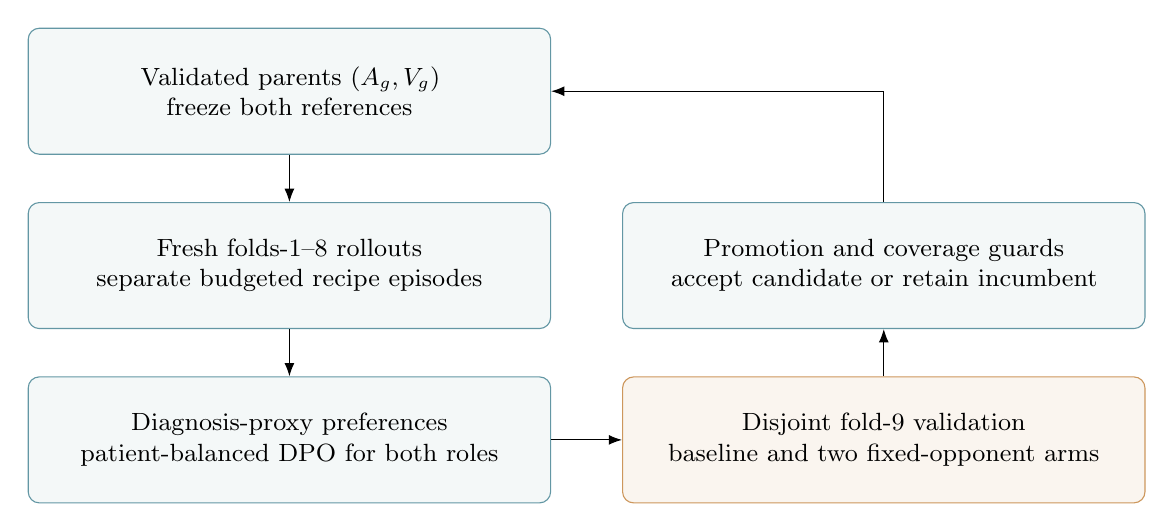
\begin{tikzpicture}[>=Latex,node distance=6mm and 9mm,
 b/.style={draw=teal!70,rounded corners,fill=teal!5,align=center,text width=64mm,minimum height=16mm,font=\small}]
 \node[b] (parents) {Validated parents $(A_g,V_g)$\\freeze both references};
 \node[b,below=of parents] (collect) {Fresh folds-1--8 rollouts\\separate budgeted recipe episodes};
 \node[b,below=of collect] (fit) {Diagnosis-proxy preferences\\patient-balanced DPO for both roles};
 \node[b,right=of fit,fill=orange!7,draw=orange!70] (validate) {Disjoint fold-9 validation\\baseline and two fixed-opponent arms};
 \node[b,above=of validate] (select) {Promotion and coverage guards\\accept candidate or retain incumbent};
 \draw[->] (parents)--(collect);\draw[->] (collect)--(fit);\draw[->] (fit)--(validate);
 \draw[->] (validate)--(select);\draw[->] (select.north) |- (parents.east);
\end{tikzpicture}
\caption{Bounded policy co-evolution. The return path uses selected incumbents; completing optimization does not imply automatic deployment of the candidate. Fold 10 is outside this loop.}
\label{fig:evolution}\end{figure}

\subsection{Checkpoint contracts and reproducible deployment}
Policies use JSON checkpoints containing feature names, action order, role, class-label order, weights, biases, and a functional policy SHA-256. Shape and finite-value checks precede deployment. The full checkpoint-file SHA-256 is separate from the functional hash, so metadata changes are also detectable when files are bound into a protocol. Expected labels and victim-model identity are checked; metadata can bind a checkpoint to its trained victim model tree.

The existing security runner loads policy files once, applies the learned verifier to every selected attack arm, and uses the learned attacker for a configured F3 arm. Both full-file and functional hashes are stored in the resolved protocol and validation lock. A held-out replay must match the locked identities; replacing a checkpoint or omitting a configured binding is rejected. This documents the current corrected binding implementation. An earlier development lock omitted the new field and is not used as the verified integration evidence here.

Each generation writes references, preferences, candidate checkpoints, evaluation, collection counts, and sealed query evidence to a new output directory. Only a completed, seal-verified run exports its final validated incumbents with completed status; failures retain an incomplete manifest and error. Trained candidate files and exported incumbents are separate artifacts. The learned wrapper supports experimental E1 execution; its existence does not satisfy E5's existing exact-built-in-attack attestation or establish a matched-coverage clinical defense comparison.

\section{DPO development experiments and observed results}
\label{sec:dporesults}
\subsection{Executed protocol and cohort}
The verified run used the existing internal PTB-XL victim, the amplitude constraint at 0.02~mV, T1 only, seed~42, and explicit limits of six training and six validation patients. All matching records for those patients were retained: seven training ECG/target cases and nine validation cases, with no patient overlap. Training uses folds 1--8 and validation fold 9. The run completed two rounds, eight gradient steps per attack, one query per recipe episode, one restart, three collection recipes, and 40 DPO epochs with $\beta=0.5$ and learning rate 0.03. These settings deliberately establish execution and audit behavior at small scale; they are not the uncapped default experiment.

\begin{table}[htbp]\centering\scriptsize
\begin{tabular}{lrrrrrrr}
\toprule
Round & Role & Pairs & Patients & Initial & Best & Pref. \% & Promoted \\
\midrule
1 & attacker & 14 & 4 & 0.693147 & 0.105057 & 92.86 & No \\
1 & verifier & 22 & 6 & 0.693147 & 0.421950 & 63.64 & No \\
2 & attacker & 14 & 4 & 0.693147 & 0.105057 & 92.86 & No \\
2 & verifier & 22 & 6 & 0.693147 & 0.405486 & 59.09 & No \\
\bottomrule
\end{tabular}

\caption{Actual frozen-reference DPO fitting in the two-round development run. Preference accuracy is a training-pair statistic, not diagnostic accuracy or validation ASR. ``Best'' denotes the restored lowest patient-balanced training loss. No candidate was promoted.}
\label{tab:dpofit}\end{table}

Attacker fitting uses 14 preferences from four training patients per round; verifier fitting uses 22 preferences from six patients. The other patients do not necessarily supply a non-tied attacker action comparison. Attacker loss decreases from 0.693147 to 0.105057 in both rounds. Verifier loss decreases to 0.421950 and 0.405486. The report independently reconstructs these four final losses from the archived feature vectors, reference/candidate checkpoints, and patient/hardness weights, without training any policy. The reconstructed values agree within $10^{-9}$.

\fig{dpo_training}{1.0}{Saved training-loss trajectories, including the initial $\log2$ state. Round-1 and round-2 attacker curves overlap. Lower training loss establishes optimization of the preference objective; it does not establish validation improvement. Curves are from the frozen run artifacts, not synthesized example data.}

\subsection{Validation, non-promotion, and stopping}
Every validation arm in both rounds has released-target ASR 0\%, diagnosis-proxy false release 100\%, and correct-clean coverage 100\%. Each arm makes 15 full pipeline calls: nine clean calls and six attack submissions for the six clean-correct ECG cases. Three queried snapshots have incorrect diagnoses; these were wrong clean reports rather than successful target attacks in this small run. The 100\% false-release metric is conditional on those wrong snapshots and averaged by patient; it is not a false-positive rate over all nine cases or a prospective population estimate.

\begin{table}[htbp]\centering\scriptsize
\begin{tabular}{lrrrrr}
\toprule
Round & Validation arm & Target \% & False release \% & Coverage \% & Calls \\
\midrule
1 & baseline & 0.0 & 100.0 & 100.0 & 15 \\
1 & attacker cand. & 0.0 & 100.0 & 100.0 & 15 \\
1 & verifier cand. & 0.0 & 100.0 & 100.0 & 15 \\
2 & baseline & 0.0 & 100.0 & 100.0 & 15 \\
2 & attacker cand. & 0.0 & 100.0 & 100.0 & 15 \\
2 & verifier cand. & 0.0 & 100.0 & 100.0 & 15 \\
\bottomrule
\end{tabular}

\caption{Separate fold-9 development validation of incumbents and candidates. Target is released-target-claim ASR, false release is the diagnosis-only proxy on wrong queried diagnoses, and coverage is correct-clean release. The baseline and each candidate are compared against the same opposing incumbent. All arms contain nine cases from six patients.}
\label{tab:dpovalidation}\end{table}

The attacker cannot pass its strict improvement rule when target ASR remains zero. The verifier retains clean coverage but cannot pass when false release is unchanged at one. Both roles therefore receive \emph{no validated gain}; no candidate is promoted in either round, and the two-round patience rule stops the loop. The exported \code{attacker.json} and \code{verifier.json} remain the initial validated priors. The round-specific candidate checkpoints contain genuinely changed weights and are retained for inspection. Describing those exported priors as an improved trained deployment would misstate the selection outcome.

Each round uses 22 collection calls plus three 15-call validation arms, or 67 waveform calls. Two rounds account for 134 waveform artifacts. The sealed training log has 136 records, including round records, and verifies complete. These costs expose the additional training exploration and validation work instead of hiding it inside the one-query per-recipe budget.

Training preference accuracy also requires care. The attacker reaches 92.86\%; verifier accuracy is 63.64\% in round 1 and 59.09\% in round 2. The latter decreases while weighted relative-preference loss falls further, because hardness weighting, parent-relative margins, and unweighted absolute preference accuracy measure different properties. None of these training statistics alone supplies evidence of a better report gate on independent patients.

\subsection{Trained-candidate runtime integration}
A separate integration check explicitly loads the trained round-1 attacker and verifier candidates into \code{security-run}; it does not replace the selected incumbent files. The check runs PGD and learned F3 K3 on the same four eligible ECG cases from two selected patients, using T1, seed~42, $B=1$, the amplitude constraint, four gradient steps, and one restart. Nine candidate clean cases are examined. Eight E1 attack submissions plus nine E0 calls yield 17 waveform artifacts; the sealed log contains 25 records and verifies complete.

Both arms have zero target and zero untargeted successes in this four-case check, and all eight selected attack submissions satisfy the amplitude constraint. These counts are integration results, not a powered comparative study.\par

Both trained checkpoint file hashes and both functional policy hashes are present in the final corrected validation lock. The report checks them against the actual candidate files and verifies that the lock binds the runtime-result digest. This establishes checkpoint loading, real queries, audit continuity, and protocol binding. It does not establish that the candidates beat their incumbents or pass the co-evolution promotion rules. The classifier, clinical primary eligibility rules, and label teacher remain the same.

\subsection{What these experiments establish and what remains open}
The completed experiments demonstrate two-role preference optimization, patient-disjoint collection and selection, a functioning adaptive gate surrogate, real waveform attack execution, explicit collection cost, rollback, patience stopping, and checkpoint-bound E1 replay. They provide a negative performance finding: the tested DPO candidates did not improve the declared validation metrics. This finding belongs in the results alongside loss reductions.

No uncapped full-patient DPO run, multi-seed DPO learning study, independent held-out DPO comparison, clinician preference collection, token-level LLM DPO, or recursive classifier training was executed. A larger study should predefine both endpoint-specific patient denominators, collection budgets, action coverage, fresh validation or nested selection, independent test isolation, and coverage-matched defense evaluation. Include frozen-prior, supervised action-classification, unweighted DPO, no-hardness, single-round, fixed-recipe, and separately trained-role controls to determine whether any eventual gain arises from the DPO objective, data collection, action selection, or gate capacity. These are proposed experiments, not rows with invented outcomes.

\clearpage


\section{Interpretation, limitations, and remaining experiments}
\label{sec:discussion}
\subsection{What the results support}
The strongest completed classification evidence is a reproducible, record-aligned fixed-candidate evaluation over the whole eligible prepared PTB-XL fold-10 cohort. The released stack improves on the previous repository run and exposes a concrete remaining weakness in HYP. The specialist result provides a useful negative finding: a large validation search can yield a modest validation gain that does not survive evaluation. The report's patient-cluster reanalysis preserves repeated-record dependence while quantifying uncertainty for frozen predictions.

The system also demonstrates an auditable composition of encoding, a learned Bayesian component, constrained state-edit search, evidence retrieval, and deterministic reporting. Explanatory evidence is scoped explicitly. However, the final probability source and the graph are different components, so interpretability of one cannot be transferred automatically to the other. The zero fused-attribution availability is the correct recorded result for this deployment configuration.

The security package demonstrates full-system query accounting, constraint validation, structured event logs, and repeatable automated outcomes. Its current results show that low-amplitude valid perturbations can alter the internal victim's predictions in a small selected cohort while reports still satisfy lexical checks. This is evidence of an engineering failure mode under a specified threat model. It is not evidence about prospective clinical impact, all-patient risk, or the external stack's robustness.

The v2 study adds a modest exact-target development gain on one constraint, with a tie on the other and no uniform untargeted advantage. The DPO study demonstrates actual optimization and correctly refuses promotion when validation metrics do not improve. Loss reduction and improved attack or verifier performance are separate results.\par

\subsection{Main threats to validity}
\textbf{Task and dataset shifts.} Single-label projection removes concurrent diagnoses and excludes unannotated rows from supervised metrics. Different PTB-XL versions do not create independent patients. MIMIC inference would involve hospital, population, acquisition, and annotation shifts. No external-site result is available.

\textbf{Model-selection uncertainty.} Validation is reused for early stopping, calibration, stack search, and extensive specialist screening. Stack cross-fitting applies only to fixed source outputs. Post-lock refit changes one source distribution. The frozen fold-10 candidate is auditable, but earlier aggregate test knowledge precludes a globally untouched-test claim. Bootstrap intervals do not account for these sources of optimism.

\textbf{Causal interpretation.} Anonymous latent factors, ordered observational graph learning, factorized priors, and directed paths do not identify physiological causal mechanisms. The ontology has no reviewed causal priors. State edits condition a learned distribution and are not physical interventions. No biomarker anchoring, interventional validation, or independent causal-graph recovery score is supplied.

\textbf{Report evaluation.} Template text is easier to cover lexically than free-form clinical language. Fact coverage can be perfect with a wrong diagnosis; the observed 500 wrong passes demonstrate this limitation. Context and semantic relevance are lexical proxies. The completed run has no real history, fallback, or abstention examples, and no clinician grading or original-paper LLM report generation.

\textbf{Security sample and endpoint.} Ten selected patients per split are inadequate for broad prevalence or rare-event conclusions. Repeated seeds and arms are dependent. Adult status and independently preserved target findings are missing. The clinical primary endpoint and all corresponding primary attack comparisons are not evaluable. Local numerical validity should never be renamed clinical preservation.

\textbf{Adaptive policy selection.} V2 uses the same candidate pool as its pilot; fold-9 outcomes informed development. DPO repeats fold-9 selection across generations and uses a diagnosis-only automated teacher. The small action catalog, single seed, and short attacks do not establish robust learning or clinically sound rejection. No policy was promoted; final incumbent files must not be described as improved trained models.\par

\textbf{Incomplete benchmark execution.} Full-dataset acquisition support is not equivalent to full evaluation. PTB-XL~1.0.1 and released QA indexing are complete, but their full inference/evaluation is not represented in the saved headline results. MIMIC acquisition is pending. No three-dataset aggregate score or original-paper QA score is available.

\subsection{Concrete completion plan for a future study}
The following experiments are proposed, not reported outcomes. First, complete the MIMIC acquisition and checksum audit, then freeze an evaluation index with clear study/patient linkage and an authorized report-reference source. Second, define task-specific QA units, multi-turn state handling, exact-match/semantic/adjudicated scoring, generator checkpoint and decoding, and waveform-linked versus text-only strata before scoring the released source rows. Report attempted, completed, failed, skipped, and adjudicated units separately.

For classification, freeze a new protocol before using additional test feedback; consider a multi-label outcome aligned with source annotations and a fresh patient/site evaluation. Compare the waveform model, Bayesian component, and ensemble under the same outcome and record set. Calibration and abstention thresholds should be chosen on validation and evaluated once on that fresh cohort. Publish both discrimination and selective coverage/error, including minority-class uncertainty and predefined subgroup checks where metadata are available.

For explanations, anchor candidate latent coordinates to measured biomarkers with external supervision and report quantitative agreement before assigning physiological names. Evaluate retrieval recall, competing-evidence exclusion, citation correctness, report entailment, diagnosis correctness, and causal-driver agreement separately, with independent clinical review. Compare template and fixed LLM generators on the same cases and corpus rather than comparing unlike local proxies with paper semantic scores.

For security, retain an all-eligible-patient index, independently establish adult and clean-report eligibility, obtain target-specific preservation evidence per queried waveform, and lock the selection and event identities. Include calibrated random controls and all requested constraint families; re-optimize attacks for each defense under matched clean coverage. Execute E1b--E7 only when the required intervention, transfer, and authenticated-history inputs are available. Report numerical and clinical endpoints separately, with patient-level uncertainty and a declared multiplicity strategy.

\section{Reproducibility and artifact availability}
\label{sec:reproducibility}
The public code URL is \url{https://github.com/elakhatibi/CARE-ECG-Full-Datasets}. The earlier published snapshot contains source, configurations, tests, and acquisition instructions; the current adaptive-v2/DPO extensions and report are local deliverables and have not been verified as published there. Local datasets, model weights, prediction JSONL, and workbooks are separate artifacts. This report is generated in the local workspace and is a separate deliverable. Its source files, aggregate evidence, tables, and figure PDFs accompany the final PDF so its interpretation can be reviewed and rebuilt where the referenced artifacts are available.

Current software validation executes all 277 tests and 103 subtests successfully. This validates tested implementation behavior, not original-paper equivalence or medical performance. Report-specific checks verify row/label/probability contracts, patient separation, agreement with saved aggregate metrics, selected provenance hashes, per-cell security means, paired v2 case-key alignment, reconstruction of DPO loss from saved preferences, candidate/reference distinctions, runtime checkpoint-lock bindings, and successful PDF compilation. The figure environment uses the system scientific Python installation (NumPy 1.26.4 and Matplotlib 3.6.3) to avoid changing the project's NumPy/PyTorch environment; exact analysis versions are recorded in \code{evidence.json}.

The build reads existing artifacts only. It does not run training, acquire new data, tune decision offsets, or rewrite historical experiment results. Long-running dataset acquisition can continue independently; data availability is a snapshot rather than a promise that pending work has completed. Appendix~\ref{app:replay} provides the operational replay sequence, and Appendix~\ref{app:provenance} identifies the main evidence files and full digests.

\section{Conclusions}
The implemented CARE-ECG workflow provides a detailed, inspectable path from ECGs to representations, Bayesian-component explanations, retrieved evidence, and reports. Its released diagnostic stack achieves 76.83\% accuracy and 68.25\% macro F1 on the declared eligible PTB-XL fold-10 cohort, with a retrospective patient-cluster macro-F1 interval of 65.45--70.90\%. Minority-class performance, selection reuse, and protocol differences remain substantial limitations. Perfect lexical report scores coexist with 500 wrong diagnoses, and the graph's explanatory scope does not extend to the external diagnostic posterior.

The locked security experiment supplies a small, reproducible automated attack benchmark for the internal waveform model, with a 25\% cell-average exact-target success rate and reduced robust accuracy at larger complete-system budgets. Clinical incorrect release is not evaluable with the present independent evidence. Full-dataset support is implemented and two source indexes are complete; MIMIC and full QA evaluation remain unfinished. Adaptive v2 adds one exact-target success in a 19-patient amplitude-constrained validation sample; spectral target rates tie. Two-role DPO reduces preference loss in two rounds but yields zero promotions. No held-out DPO improvement or clinical verifier benefit is established. These distinctions preserve the usefulness of the measured results without turning missing experiments or implementation choices into original-paper reproduction claims.

\clearpage

\appendix
\section{Notation and implementation map}
\label{app:notation}
\begin{longtable}{p{0.18\linewidth}p{0.74\linewidth}}
\toprule Symbol & Meaning in this implementation\\\midrule\endhead
$x,x'$ & Raw-mV and globally standardized multilead ECG, respectively.\\
$C,T,N$ & Lead count, time samples per record, and number of records.\\
$h,z,\mu,\sigma$ & Pooled encoder feature, stochastic latent sample, posterior mean, and posterior standard deviation.\\
$\tilde z$ & Per-coordinate categorical state from training quantiles.\\
$y,\hat y,y^*$ & Projected reference superclass, predicted class, and requested target.\\
$p_{\mathrm{BN}}$ & Internal Bayesian-network posterior conditioned on latent states.\\
$p_{\mathrm{neural}}$ & Internal supervised waveform classifier probabilities.\\
$p_{\mathrm{stack}}$ & External locked stack probabilities from three aligned sources.\\
$w_n,w_e$ & Internal neural-fusion and external-expert weights; both are 1 in the released diagnostic run.\\
$\mathcal{S}_j$ & Empirically supported categorical states of latent coordinate $j$.\\
$R,e,q$ & Retrieved facts, generated explanation, and query.\\
$\delta,\mathcal{S}$ & Raw-mV waveform perturbation and its declared feasible set.\\
$B,\kappa$ & Maximum complete-system attack submissions and targeted log-score confidence margin.\\
OOF & Out-of-fold stacker predictions on grouped partitions of validation fold~9.\\
ASR & Attack success rate for a specified outcome, conditioning rule, budget, and victim.\\
\bottomrule
\end{longtable}

\begin{longtable}{p{0.43\linewidth}p{0.49\linewidth}}
\toprule Source module & Main responsibility\\\midrule\endhead
\code{src/care_ecg/data.py} & Lead orientation, finite repair, resampling, crop/pad, normalization, PTB-XL label preparation.\\
\code{src/care_ecg/models.py} & Temporal backbones, VAE posterior/decoder, supervised classification and loss.\\
\code{src/care_ecg/training.py} & Augmentation, optimization, early stopping, validation fusion and class biases.\\
\code{src/care_ecg/discretization.py} & Training-quantile thresholds and categorical transformation.\\
\code{src/care_ecg/causal.py} & Ordered K2/BDeu structure, CPTs, exact inference, drivers and paths.\\
\code{src/care_ecg/counterfactual.py} & Exhaustive supported single-coordinate state edits and scoped result.\\
\code{src/care_ecg/pipeline.py} & Training composition, deterministic batch encoding, agent orchestration, save/load.\\
\code{src/care_ecg/agents.py} & History, diagnosis, response prompts, fallback, causal retrieval coordination.\\
\code{src/care_ecg/retrieval.py} & TF-IDF/optional embeddings, enriched query, metadata scores, competing-class filter.\\
\code{src/care_ecg/generation.py} & Deterministic template and optional local/API generator adapters.\\
\code{src/care_ecg/verification.py} & Retrieved-fact coverage and citation/claim-support lexical checks.\\
\code{src/care_ecg/ensemble.py} & Hash-authenticated legacy adapters, SCP features, grouped stacker and strict alignment.\\
\code{src/care_ecg/finalization.py} & Frozen-source recomputation, offsets, final expert manifest.\\
\code{src/care_ecg/metrics.py} & Categorical, Text-to-SCP, lexical grounding and wrong-diagnosis gate metrics.\\
\code{src/care_ecg/reporting.py} & Workbook exports, comparison targets, reproduction attestation.\\
\code{src/care_ecg/paper_data.py} & Versioned acquisition, locks, integrity checks and all-source indexing.\\
\code{src/care_ecg/paper_inference.py} & Streaming all-record inference, WFDB units, QA linkage and text-only path.\\
\path{src/care_ecg/security/preferences.py} & Finite-action policies, JSON contracts, frozen-reference DPO and patient weighting.\\
\path{src/care_ecg/security/learned.py} & Recipe selector, waveform/report features, veto gate and differentiable surrogate.\\
\path{src/care_ecg/security/evolution.py} & Fresh collection, disjoint validation, promotion, rollback and sealed generation logs.\\
\path{src/care_ecg/security/evolution_cli.py} & Fold-enforced, all-matching-record training runner and input provenance.\\
\code{src/care_ecg/security/} & Threat contracts, attacks, waveform constraints, defenses, endpoints, uncertainty and logs.\\
\bottomrule
\end{longtable}

\section{Operational algorithms}
\label{app:algorithms}
The following pseudocode describes the implemented data flow. Its labels are software variables, not independently validated physiological mechanisms.

\subsection{Fit the internal representation and graph}
\begin{lstlisting}
Input: train ECGs/labels, explicit validation ECGs/labels, frozen config
1. Fit global mean/scale on train only; transform both splits.
2. Train supervised temporal VAE with denoising augmentation and KL warm-up.
3. Select early-stopping epoch on validation macro F1; restore weights.
4. Encode training ECGs with posterior means, without stochastic sampling.
5. Fit coordinate quantiles on training means; discretize training means.
6. Learn ordered graph with K2/BDeu and declared prior-edge constraints.
7. Estimate smoothed CPTs from training states and labels.
8. Evaluate candidate neural/BN mixtures and class offsets on validation.
9. Fit the configured retrieval index from the versioned knowledge documents.
Output: weights, config, normalizer, discretizer, network, retrieval index,
        training history and validation-selection diagnostics.
\end{lstlisting}

\subsection{Released diagnostic/report execution}
\begin{lstlisting}
Input: ECG batch, queries, optional history, aligned expert probabilities
1. Apply saved preprocessing and normalization.
2. Encode posterior mean and internal neural probabilities in one pass.
3. Validate external rows, label order, probabilities, source and hashes.
4. Blend external/internal neural probabilities using locked expert weight.
5. Discretize mean; compute Bayesian and fused diagnosis posteriors.
6. Select label, scoped sensitivity drivers and directed paths.
7. If requested, search supported single-factor target-state edits.
8. Choose latest supplied same-patient history or labeled latent surrogate.
9. Enrich query; rank eligible knowledge; retain retrieved fact provenance.
10. Build fact-tagged prompt and deterministic/generated draft.
11. Check retrieved-fact coverage and unsupported claims.
12. If needed, retry without causal fields; then use evidence-only fallback.
13. Return probabilities, label, rationale, scopes, facts and audit states.
14. Append expected label only for evaluation bookkeeping.
\end{lstlisting}

\subsection{Attack and count complete-system queries}
\begin{lstlisting}
Input: clean-correct case, target, constraint, frozen attack and budget B
1. Bind clean snapshot, patient/record identity, verifier and raw-mV contract.
2. For each allowed restart while query budget remains:
   a. Initialize seeded random delta and project into the declared set.
   b. Optimize the differentiable surrogate for 40 steps (locked study).
   c. Keep the minimum-surrogate-loss candidate from this restart.
   d. Submit it to the real waveform-callable pipeline; consume one query.
   e. Record diagnosis, facts, text, release, constraints and distortion.
   f. Assess independent preservation if a qualifying reviewer is supplied.
3. Derive automated any-query target/untargeted/released-claim outcomes.
4. Keep clinical-primary status separate from automated target outcomes.
5. Write selected artifacts, full query trace, hash chain and terminal seal.
Output: typed attack result and endpoint-specific evaluability.
\end{lstlisting}

\subsection{Bootstrap frozen classification outputs}
\begin{lstlisting}
Input: true/predicted labels and patient IDs for every eligible test ECG
1. Aggregate a 5 x 5 confusion matrix for each distinct patient and system.
2. Repeat 10,000 times with seed 20261027:
   a. Sample the full number of patient IDs with replacement.
   b. Sum all sampled patients' matrices, including multiplicities.
   c. Recompute accuracy, macro precision/recall/F1 for each system.
   d. Compute paired differences using the same sampled IDs.
3. Report original full-cohort metrics and percentile 95% intervals.
No model is refitted and no report or label is changed.
\end{lstlisting}

\section{Complete additional meta-model screening results}
\label{app:candidates}
\begin{table}[H]\centering\small
\begin{tabular}{lrr}
\toprule
Candidate & Standalone F1 (\%) & Added-stack F1 (\%) \\
\midrule
hist\_bal0375 & 68.33 & 69.62 \\
hist\_shallow & 68.38 & 69.57 \\
hist\_deep & 68.59 & 69.44 \\
hist\_rich & 68.16 & 69.48 \\
extra\_leaf2\_w0375 & 67.89 & 69.09 \\
extra\_leaf4\_w05 & 67.63 & 69.05 \\
extra\_sqrt\_leaf1\_w025 & 66.26 & 68.95 \\
rf\_sqrt\_leaf2\_w0375 & 67.40 & 69.07 \\
rf\_04\_leaf3\_w0375 & 66.83 & 68.92 \\
logit\_C01\_w0375 & 66.52 & 69.60 \\
logit\_C1\_w0375 & 66.18 & 69.82 \\
mlp\_128\_32\_w0375 & 66.35 & 69.10 \\
lgbm\_leaf31 & 67.31 & 69.34 \\
lgbm\_leaf15 & 68.02 & 69.49 \\
lgbm\_rich\_leaf31 & 67.27 & 69.11 \\
lgbm\_leaf63 & 67.55 & 69.23 \\
lgbm\_leaf31\_w05 & 67.84 & 69.48 \\
\bottomrule
\end{tabular}

\caption{All 17 additional validation-screened candidate sources. Standalone scores use fold-9 outputs; added-stack values are each candidate's best patient-grouped stacker OOF selection score. The released baseline is 69.876\% OOF macro F1. The candidate labels are the experiment's recorded names, not new fitted models.}
\end{table}
The closest added-stack candidate is \code{logit_C1_w0375} at approximately 69.82\% macro F1. This screening table uses the same fold-9 selection outcomes as the archived search. It is not a new ranking based on test labels. Individual comparisons are not adjusted for the number of models or hyperparameters tried.

\section{Complete locked validation attack matrix}
\label{app:securityvalidation}
\begin{table}[H]\centering\scriptsize
\resizebox{\linewidth}{!}{\begin{tabular}{llrrrr}
\toprule
Attack & Constraint & B & Target ASR (\%) [95\% CI] & Untargeted (\%) & Robust (\%) \\
\midrule
F1 PGD & L-infinity & 1 & 20.0 [0.0, 50.0] & 56.7 & 43.3 \\
F1 PGD & L-infinity & 3 & 20.0 [0.0, 50.0] & 70.0 & 30.0 \\
F1 PGD & Spectral & 1 & 10.0 [0.0, 30.0] & 20.0 & 80.0 \\
F1 PGD & Spectral & 3 & 10.0 [0.0, 30.0] & 20.0 & 80.0 \\
F1-CF & L-infinity & 1 & 20.0 [0.0, 50.0] & 36.7 & 63.3 \\
F1-CF & L-infinity & 3 & 20.0 [0.0, 50.0] & 80.0 & 20.0 \\
F1-CF & Spectral & 1 & 10.0 [0.0, 30.0] & 20.0 & 80.0 \\
F1-CF & Spectral & 3 & 10.0 [0.0, 30.0] & 20.0 & 80.0 \\
F3 K2 & L-infinity & 1 & 20.0 [0.0, 50.0] & 63.3 & 36.7 \\
F3 K2 & L-infinity & 3 & 20.0 [0.0, 50.0] & 76.7 & 23.3 \\
F3 K2 & Spectral & 1 & 10.0 [0.0, 30.0] & 20.0 & 80.0 \\
F3 K2 & Spectral & 3 & 10.0 [0.0, 30.0] & 20.0 & 80.0 \\
F3 K3 & L-infinity & 1 & 20.0 [0.0, 50.0] & 63.3 & 36.7 \\
F3 K3 & L-infinity & 3 & 20.0 [0.0, 50.0] & 76.7 & 23.3 \\
F3 K3 & Spectral & 1 & 10.0 [0.0, 30.0] & 30.0 & 70.0 \\
F3 K3 & Spectral & 3 & 10.0 [0.0, 30.0] & 30.0 & 70.0 \\
\bottomrule
\end{tabular}
}
\caption{Locked validation E1 results for the C3 configuration. Targeted ASR intervals use the saved 10,000-resample patient bootstrap. Each row is ten patients with three seeds. These rows were available during attack selection; they are not independent held-out estimates.}
\end{table}
The matrix is deliberately reported alongside held-out results. The apparent consistency of exact-target rates across attack families contrasts with varying untargeted outcomes and shows why ``attack success'' needs an explicit outcome definition. A target can fail while a different wrong diagnosis is still found.

\section{Complete held-out distortion and query results}
\label{app:distortion}
\begin{table}[H]\centering\scriptsize
\resizebox{\linewidth}{!}{\begin{tabular}{llrrrrr}
\toprule
Attack & Constraint & B & RMSE (mV) & PRD (\%) & SNR (dB) & Queries \\
\midrule
F1 PGD & s\_inf & 1 & 0.0180 & 9.5322 & 20.5434 & 30 \\
F1 PGD & s\_inf & 3 & 0.0180 & 9.5482 & 20.5297 & 90 \\
F1 PGD & s\_spec & 1 & 0.0043 & 2.2539 & 33.0175 & 30 \\
F1 PGD & s\_spec & 3 & 0.0043 & 2.2560 & 33.0096 & 90 \\
F1-CF & s\_inf & 1 & 0.0181 & 9.5803 & 20.4987 & 30 \\
F1-CF & s\_inf & 3 & 0.0181 & 9.6000 & 20.4837 & 90 \\
F1-CF & s\_spec & 1 & 0.0043 & 2.2669 & 32.9742 & 30 \\
F1-CF & s\_spec & 3 & 0.0043 & 2.2709 & 32.9589 & 90 \\
F3 K2 & s\_inf & 1 & 0.0181 & 9.5880 & 20.4950 & 30 \\
F3 K2 & s\_inf & 3 & 0.0181 & 9.5999 & 20.4854 & 90 \\
F3 K2 & s\_spec & 1 & 0.0043 & 2.2547 & 33.0148 & 30 \\
F3 K2 & s\_spec & 3 & 0.0043 & 2.2584 & 33.0002 & 90 \\
F3 K3 & s\_inf & 1 & 0.0178 & 9.4312 & 20.6314 & 30 \\
F3 K3 & s\_inf & 3 & 0.0178 & 9.4399 & 20.6249 & 90 \\
F3 K3 & s\_spec & 1 & 0.0043 & 2.2526 & 33.0232 & 30 \\
F3 K3 & s\_spec & 3 & 0.0043 & 2.2545 & 33.0153 & 90 \\
\bottomrule
\end{tabular}
}
\caption{Mean distortion of selected valid perturbations and total complete attack queries per held-out cell. PRD and SNR are averaged per selected waveform, so they should not be recomputed from a single ratio of the table's averaged norms. The selected candidate need not be the first successful or largest-distortion query.}
\end{table}
Each $B=1$ row uses 30 complete submissions and each $B=3$ row uses 90, totaling 960 attack submissions. The raw query schedule is separate from the 40-step gradient loops. All selected-constraint validity rates are 1.0, with no inference that a target-specific clinical finding has been preserved.

\section{Exploratory momentum validation matrix}
\label{app:momentum}
\begin{table}[H]\centering\scriptsize
\resizebox{\linewidth}{!}{\begin{tabular}{llrrrr}
\toprule
Attack & Constraint & B & Target ASR (\%) [95\% CI] & Untargeted (\%) & Robust (\%) \\
\midrule
F1 PGD & L-infinity & 1 & 20.0 [0.0, 50.0] & 50.0 & 50.0 \\
F1 PGD & L-infinity & 3 & 20.0 [0.0, 50.0] & 63.3 & 36.7 \\
F1 PGD & Spectral & 1 & 10.0 [0.0, 30.0] & 36.7 & 63.3 \\
F1 PGD & Spectral & 3 & 10.0 [0.0, 30.0] & 43.3 & 56.7 \\
F1-CF & L-infinity & 1 & 20.0 [0.0, 50.0] & 46.7 & 53.3 \\
F1-CF & L-infinity & 3 & 20.0 [0.0, 50.0] & 66.7 & 33.3 \\
F1-CF & Spectral & 1 & 10.0 [0.0, 30.0] & 26.7 & 73.3 \\
F1-CF & Spectral & 3 & 10.0 [0.0, 30.0] & 50.0 & 50.0 \\
F3 K2 & L-infinity & 1 & 20.0 [0.0, 50.0] & 46.7 & 53.3 \\
F3 K2 & L-infinity & 3 & 20.0 [0.0, 50.0] & 60.0 & 40.0 \\
F3 K2 & Spectral & 1 & 10.0 [0.0, 30.0] & 30.0 & 70.0 \\
F3 K2 & Spectral & 3 & 10.0 [0.0, 30.0] & 36.7 & 63.3 \\
F3 K3 & L-infinity & 1 & 20.0 [0.0, 50.0] & 46.7 & 53.3 \\
F3 K3 & L-infinity & 3 & 20.0 [0.0, 50.0] & 60.0 & 40.0 \\
F3 K3 & Spectral & 1 & 10.0 [0.0, 30.0] & 30.0 & 70.0 \\
F3 K3 & Spectral & 3 & 10.0 [0.0, 30.0] & 36.7 & 63.3 \\
\bottomrule
\end{tabular}
}
\caption{Separate momentum-decay-0.9 validation experiment. Each row has ten patients and three seeds. It is not a held-out replacement and does not share the earlier final study's historical code identity. Clinical primary evaluability remains absent.}
\end{table}
The momentum run's event verification reports a complete log with 1,398 records and 918 waveform artifacts, consistent with 888 attack queries plus 30 clean waveform evaluations. The lower query count than the earlier run does not by itself establish a more query-efficient clinical attack: the stopping path, automated outcomes, and primary eligibility have to be interpreted separately.

\section{Replaying and extending the workflow}
\label{app:replay}
The following commands are a map to the existing CLI, not a claim that all stages were rerun for this PDF. Inputs and optional dependencies must be present. Full original-paper equivalence additionally requires author artifacts or a confirmed matching protocol that is currently unavailable.

\subsection{Environment and eligible supervised cohort}
\begin{lstlisting}[language=bash]
python3 -m venv .venv
source .venv/bin/activate
python -m pip install -e '.[data,ensemble,reports,dev]'

care-ecg prepare-ptbxl data/ptb-xl data/ptbxl-prepared \
  --sampling-rate 100 --seconds 10 --normalization none

care-ecg train data/ptbxl-prepared/train.npz \
  artifacts/ptbxl-inception-validation \
  --config config/ptbxl_inception.yaml --preprocessed \
  --label-names NORM,MI,STTC,CD,HYP \
  --validation-dataset data/ptbxl-prepared/validation.npz \
  --knowledge-graph data/ptbxl-prepared/knowledge_graph.json
\end{lstlisting}
The exact external-source acquisition, hash authentication, SCP meta-model, grouped stacker selection, post-lock refit, and finalizer commands are documented in \code{scripts/README.md} and \code{REPRODUCIBILITY.md}. These steps depend on authenticated legacy probability arrays and weights; cloning the source repository alone does not supply them. Historical locks should be preserved when creating a new run rather than overwritten as if the old pre-evaluation provenance still applied.

\subsection{Replaying released fixed probabilities}
\begin{lstlisting}[language=bash]
care-ecg predict artifacts/ptbxl-nextgen-final \
  data/ptbxl-prepared/test.npz outputs/replay-test.jsonl \
  --preprocessed --batch-size 64 \
  --expert-probabilities \
    artifacts/ptbxl-benchmark/stack-three-source/test_probabilities_nextgen_locked.npz \
  --expert-weight 1.0 \
  --expert-source nextgen-three-source-stacker

care-ecg evaluate outputs/replay-test.jsonl \
  --scp-aliases data/ptbxl-prepared/scp_aliases.json \
  --scp-fuzzy-threshold 0.84
\end{lstlisting}
For an actual provenance replay, retain the original full expert-source hash string from the README and authenticate every required input against the lock. The shorter source label above is an illustrative CLI invocation, not a substitute for source authentication. Expected labels used for bookkeeping must remain outside prediction decisions.

\subsection{All-source indexing and inference}
\begin{lstlisting}[language=bash]
care-ecg prepare-paper-data

# Completed paper-count PTB-XL source index:
care-ecg predict-paper artifacts/ptbxl-nextgen-final \
  data/paper-prepared/ptbxl.jsonl data/ptb-xl-1.0.1 \
  outputs/ptbxl-101-all-records.jsonl

# Same waveform-callable path, filtered to a declared test fold:
care-ecg predict-paper artifacts/ptbxl-nextgen-final \
  data/paper-local-prepared/ptbxl.jsonl data/ptb-xl \
  outputs/internal-waveform-fold10.jsonl --folds 10

# Once MIMIC acquisition/indexing is complete:
care-ecg answer-expert-qa artifacts/ptbxl-nextgen-final \
  data/paper-prepared/expert-qa.jsonl outputs/qa-all.jsonl \
  --mimic-index data/paper-prepared/mimic.jsonl \
  --mimic-root data/mimic-iv-ecg-1.0
\end{lstlisting}
The first all-record waveform command includes training records. The second still uses the internal waveform model, so its probabilities need not match the cached external-stack headline even on the same fold. The QA command preserves references for adjudication and distinguishes linked-waveform and text-only cases; it does not produce a paper-comparable QA score automatically. Existing output files are not reused silently because full-corpus writers use exclusive creation.

\subsection{New all-patient security study}
\begin{lstlisting}[language=bash]
care-ecg security-run artifacts/ptbxl-nextgen-final \
  data/ptbxl-prepared/validation.npz outputs/security-all-validation \
  --all-patients --records-per-patient all
\end{lstlisting}
This removes caps for a new study and retains all matching eligible ECGs, while preserving target eligibility and fold rules. It does not supply independent adult or preservation adjudication. A held-out extension must use an appropriate newly frozen validation lock and historical input identities; the archived small-cohort result should not be renamed after changing these settings.

\subsection{Exact adaptive-v2 development replay}
\begin{lstlisting}[language=bash]
OMP_NUM_THREADS=2 MKL_NUM_THREADS=2 care-ecg security-run \
  artifacts/ptbxl-nextgen-final \
  data/ptbxl-prepared/validation.npz \
  results/security-adaptive-v2-expanded-replay \
  --security-config config/security_ptbxl_adaptive_v2_validation.yaml \
  --phase validation --budgets 1 --seeds 42 \
  --max-eligible-per-target 30
\end{lstlisting}
The eligible cap of 30 permits all 19 clean-correct patients from the original 30-candidate pool. Omitting these explicit overrides changes the measured study: the configuration otherwise defaults to ten eligible patients, two budgets, and three seeds. Use a fresh output path and the original source identity for exact historical replay; current source identities are separately recorded.

\subsection{Exact two-round DPO development command}
\begin{lstlisting}[language=bash]
care-ecg security-evolve artifacts/ptbxl-nextgen-final \
  data/ptbxl-prepared/train.npz \
  data/ptbxl-prepared/validation.npz \
  artifacts/security-dpo-evolution-replay \
  --rounds 2 --steps 8 --dpo-epochs 40 --targets T1 \
  --max-train-patients-per-target 6 \
  --max-validation-patients-per-target 6

# Uncapped matching-patient configuration for a future run:
care-ecg security-evolve artifacts/ptbxl-nextgen-final \
  data/ptbxl-prepared/train.npz \
  data/ptbxl-prepared/validation.npz \
  artifacts/security-dpo-evolution-full \
  --evolution-config config/security_evolution.yaml
\end{lstlisting}
The first command reproduces the declared development limits, not a promise of improvement. The second command is a proposed full matching-patient run and has not been executed for the results in this report. Neither command accepts fold 10 as training or selection data. The output directory must be new and outside the immutable victim-artifact directory.

\begin{table}[htbp]\centering\small
\begin{tabular}{lrr}
\toprule Setting & Default evolution & Measured development\\\midrule
Rounds / patience & 3 / 2 & 2 / 2\\
DPO epochs / learning rate & 80 / 0.03 & 40 / 0.03\\
Beta / gradient clip & 0.5 / 1.0 & 0.5 / 1.0\\
Gradient steps / restarts & 40 / 1 & 8 / 1\\
Queries per recipe / collection recipes & 1 / 3 & 1 / 3\\
Perturbation amplitude (mV) & 0.02 & 0.02\\
Maximum retained preference pairs & No cap & No cap\\
Patients per target per split & No cap & 6\\
Matching records per patient & All & All\\
Correct-clean coverage floor & 0.90 & 0.90\\
Maximum clean coverage drop & 0.02 & 0.02\\
Minimum metric improvement & 0.0001 & 0.0001\\\bottomrule
\end{tabular}
\caption{Evolution defaults versus actually executed development settings. The minimum improvement is an empirical selection threshold, not a confidence level.}
\end{table}

\subsection{Applying selected or experimental candidate policies}
After training, the configured final files select validated incumbents, which can remain priors. To reproduce a trained-candidate integration check, explicitly use the round-specific candidate paths and label that choice experimental. A minimal configuration extension is:
\begin{lstlisting}
protocol:
  verifier_policy: artifacts/security-dpo-evolution/verifier.json
attacks:
  f3_k3:
    preference_policy: artifacts/security-dpo-evolution/attacker.json
    defense_weight: 1.0
\end{lstlisting}
Merge these fields into a complete versioned security configuration; they are not a standalone protocol. Preserve the dataset/model hashes, constraints, comparators, seeds, and budgets. Run validation to generate a new checkpoint-bound lock before any held-out replay. A wrapper's valid E1 result does not waive requirements of the separate E5 attestation API.

\subsection{Rebuilding this report}
From the repository root, using the compatible scientific Python and local TeX installation:
\begin{lstlisting}[language=bash]
/usr/bin/python3 reports/methodology-20261028/build_evidence.py
cd reports/methodology-20261028
pdflatex -interaction=nonstopmode -halt-on-error \
  -jobname=CARE_ECG_Detailed_Methodology_and_Results manuscript.tex
pdflatex -interaction=nonstopmode -halt-on-error \
  -jobname=CARE_ECG_Detailed_Methodology_and_Results manuscript.tex
\end{lstlisting}
The builder checks existing cohort/prediction alignment and metric consistency, writes aggregate JSON/CSV/TeX, and exports vector figures with raster previews. A fresh rebuild after a dataset manifest changes should be treated as a new status snapshot and checked against the prose. The manuscript is not an automatic claim generator for uncompleted experiments.

\section{Evidence ledger and provenance}
\label{app:provenance}
The classification ledger consists of \code{results/CARE_ECG_nextgen_run_metadata.json}, the pre-inference selection lock, \code{outputs/ptbxl-nextgen-ensemble-test.jsonl}, the final artifact, and the aligned prepared archives. The prior-run and specialist JSONL files support paired reanalysis. Security evidence comes from the final C3 validation and held-out \code{security_results.json} files and their sealed event packages; momentum validation is a separate source. Acquisition status comes from \code{data/paper-prepared/manifest.json} and the local all-record manifest.

The report builder explicitly verifies the saved classification model, stacker, selection-lock, and final-prediction digests against the original metadata. It checks source record alignment, labels, finite normalized probabilities, predicted argmax, no patient overlap, and agreement of the rebuilt metrics. It also checks that each security summary point matches the raw observation mean for its cell. It imports saved security integrity receipts; it does not independently rerun clinical adjudication or rehash every archived waveform.

Full input digests and current Python-source digests are in the accompanying \code{evidence.json}. Historical code-tree identities embedded in security results remain distinct from the current source snapshot. The following key digests make the main numerical sources independently identifiable.
\begin{longtable}{p{0.55\linewidth}p{0.38\linewidth}}
\toprule
Input artifact & SHA-256 (two consecutive halves) \\
\midrule\endhead
{\scriptsize\path{artifacts/ptbxl-nextgen-final/causal_vae.pt}} & {\scriptsize\ttfamily ae32c49fa341fede8c503cd055df6d39\newline 648582197fa95edd8fced533827b2fad} \\
{\scriptsize\path{artifacts/ptbxl-benchmark/stack-three-source/locked_probability_stacker.npz}} & {\scriptsize\ttfamily 09d52edf2dcffb24d41cfc442b8bb7eb\newline d1bfcdeeb3138064d58dad3f7b3e2429} \\
{\scriptsize\path{results/CARE_ECG_nextgen_locked_selection.json}} & {\scriptsize\ttfamily fc5f38167c35bd7f3e99d4433f68724f\newline 7db18f670d7a96a9329639c245410889} \\
{\scriptsize\path{outputs/ptbxl-nextgen-ensemble-test.jsonl}} & {\scriptsize\ttfamily c4adfd3bc242c080fd17ec3d49686cc7\newline ee4bb62a3bc559cfe6aa762fa3375ecc} \\
{\scriptsize\path{data/ptbxl-prepared/test.npz}} & {\scriptsize\ttfamily fd90c55c047d5f37a196e98aa127a836\newline 29eecd4622c653653fd9511cc33c1868} \\
{\scriptsize\path{results/security-final-validation-c3-b1-b3-s3-20261026/security_results.json}} & {\scriptsize\ttfamily 5ed1c253df1f4356ec2bb73dd5bd4e0f\newline 07b7712604fa5482a698cee4312af737} \\
{\scriptsize\path{results/security-final-heldout-c3-b1-b3-s3-20261026/security_results.json}} & {\scriptsize\ttfamily 83dd22d00cd860cc0cc7832348f90f53\newline 95252f0c4e1f2465f4468959dc6b3eb8} \\
{\scriptsize\path{results/security-mipgd-validation-20261026/security_results.json}} & {\scriptsize\ttfamily 2d704ac3c48f676e21b27716ce82ede2\newline 0e6b18a993a41a763ed995456bd753d5} \\
{\scriptsize\path{data/paper-prepared/manifest.json}} & {\scriptsize\ttfamily c529ac99fd59a9115477e61e0a91978a\newline 548ee834923cb3827ae506341bfcf9a4} \\
\bottomrule
\end{longtable}


Adaptive-v2 and DPO artifacts have their own historical source identities. The following additional inputs support the new sections; preference records are read only for aggregate loss verification and are not embedded in the report package. The current source hashes and all checked input digests are in \code{evidence.json}.
\begin{longtable}{p{0.55\linewidth}p{0.38\linewidth}}
\toprule
New experiment input & SHA-256 (two consecutive halves) \\
\midrule\endhead
{\scriptsize\path{results/security-adaptive-v2-expanded-validation-20261028/security_results.json}} & {\scriptsize\ttfamily 1f37a5fc9846bec2625fbbfaf8cf8229\newline e48ae4d2d94b6c2d1c1fff5003b45a30} \\
{\scriptsize\path{results/security-adaptive-v2-expanded-validation-20261028/adaptive_v2_comparison_summary.json}} & {\scriptsize\ttfamily f96a72bb3afab46d59a215e9920fedee\newline 88750d38134533938823bb05efeeeb2d} \\
{\scriptsize\path{artifacts/security-dpo-evolution-verified-20261028/manifest.json}} & {\scriptsize\ttfamily d94440e3cc996775f18b5730972aecf9\newline 6c3a3eff7c242e2cdaabe476bb5f1fd1} \\
{\scriptsize\path{results/security-dpo-final-binding-check-20261028/security_results.json}} & {\scriptsize\ttfamily 0a940f2f35cc76f54de4f08ebf5cfacd\newline 1a959a1b7e49aaef533e7b9140f6a3cc} \\
{\scriptsize\path{results/security-dpo-final-binding-check-20261028/security_protocol.lock.json}} & {\scriptsize\ttfamily efc3960db0f369b2160024a0b9510bba\newline d770342ff0f3c70023994c20cc10c1e6} \\
{\scriptsize\path{artifacts/security-dpo-evolution-verified-20261028/round-001/attacker-candidate.json}} & {\scriptsize\ttfamily 93ad75be02cb5aadd99f66fbb28b886f\newline bb5b26613dc683906bf96d71fbd4832d} \\
{\scriptsize\path{artifacts/security-dpo-evolution-verified-20261028/round-001/verifier-candidate.json}} & {\scriptsize\ttfamily c7965e733f633caf8cdfe067fbc0b33a\newline c06761ebef44e4e2775613aac007cf11} \\
\bottomrule
\end{longtable}


\section{Result-status checklist}
\label{app:status}
\begin{longtable}{p{0.50\linewidth}p{0.42\linewidth}}
\toprule Item & Evidence status at report snapshot\\\midrule\endhead
Eligible PTB-XL categorical fold-10 predictions & Complete: 2,158 ECGs / 1,877 patients.\\
Released-stack aggregate metrics and class errors & Measured; independently recovered from frozen outputs.\\
Patient-cluster classification intervals and paired differences & New retrospective fixed-prediction reanalysis; 10,000 resamples.\\
Waveform-specialist improvement study & Complete; not promoted after one locked candidate evaluation.\\
Template lexical report proxies & Measured; not clinical or paper-exact semantic outcomes.\\
Longitudinal report improvement & Not evaluated in released classification run (history mode none).\\
Physiological causal latent identification & Not established; anonymous factors and observational state edits.\\
Expanded C3 validation and held-out attacks & Complete small-cohort E0/E1 automated study.\\
Clinical incorrect-release primary endpoint & Not evaluable; independent eligibility/preservation evidence missing.\\
Full-population adversarial study & Not completed; historical locked cohort capped at ten selected patients.\\
Adaptive v2 nine-attack comparison & Validation only: 19 patients; modest amplitude target gain; spectral tie.\\
Two-role frozen-reference DPO & Two small real-data rounds; actual fitting, zero promotions.\\
DPO trained-candidate E1 integration & Checkpoint loading and lock binding verified; not promotion evidence.\\
Full-cohort or held-out DPO gain & Not evaluated.\\
Momentum attack extension & Validation-only exploratory evidence; no new held-out result.\\
V2/V3 matched-coverage and E1b--E7 effects & Implemented APIs; no completed primary effect estimate in this report.\\
PTB-XL~1.0.1 full source & Downloaded, verified and indexed: 21,837 ECGs / 18,885 patients.\\
Local all-record PTB-XL source & Indexed: 21,799 ECGs / 18,869 patients, including unlabeled records.\\
Released Expert-ECG-QA source & Indexed: 43,670 source rows / 11 files; 17,024 identifiable patients.\\
MIMIC-IV-ECG full source & Acquisition pending in snapshot manifest.\\
Full QA task-specific benchmark metrics & Not completed; released-row normalization and runner available.\\
Original CARE-ECG exact reproduction & NOT REPRODUCED.\\
\bottomrule
\end{longtable}

\clearpage
\begin{thebibliography}{30}
\small
\setlength{\itemsep}{3pt}
\addcontentsline{toc}{section}{References}
\bibitem{care} E. Khatibi, Z. Wang, A. Sharma, K. Chakrabarty, S. Rahimi Moosavi, F. Firouzi, and A.-M. Rahmani.
\emph{CARE-ECG: Causal Agent-based Reasoning for Explainable and Counterfactual ECG Interpretation}. arXiv:2604.10420, 2026. Original architecture and reference results; local supplied PDF reviewed alongside the repository. \url{https://arxiv.org/abs/2604.10420}.
\bibitem{ptbxl} P. Wagner et al. \emph{PTB-XL, a large publicly available electrocardiography dataset}. Scientific Data 7, 154, 2020. \url{https://doi.org/10.1038/s41597-020-0495-6}.
\bibitem{ptbxl_data} P. Wagner et al. \emph{PTB-XL}, version 1.0.3. PhysioNet, 2022. Release metadata and recommended folds. \url{https://physionet.org/content/ptb-xl/1.0.3/}.
\bibitem{ptbxl_old} P. Wagner et al. \emph{PTB-XL}, version 1.0.1. PhysioNet. Acquisition version chosen for paper-count coverage, separately from the completed local supervised experiment. \url{https://physionet.org/content/ptb-xl/1.0.1/}.
\bibitem{mimic} B. Gow et al. \emph{MIMIC-IV-ECG: Diagnostic Electrocardiogram Matched Subset}, version 1.0. PhysioNet, 2023. DOI:10.13026/4nqg-sb35. \url{https://physionet.org/content/mimic-iv-ecg/1.0/}.
\bibitem{qa} X. Wang et al. \emph{ECG-Expert-QA: A Benchmark for Evaluating Medical Large Language Models in Heart Disease Diagnosis}. arXiv:2502.17475, 2025. \url{https://arxiv.org/abs/2502.17475}.
\bibitem{qa_repo} Zaozzz/ECG-Expert-QA. Publisher dataset repository; pinned revision \code{4fcb46974eed422532772caa483a5e621f006ff1}. Local count audit uses that revision, not a mutable current branch. \url{https://github.com/Zaozzz/ECG-Expert-QA}.
\bibitem{inception} H. Ismail Fawaz et al. \emph{InceptionTime: Finding AlexNet for Time Series Classification}. Data Mining and Knowledge Discovery, 2020; arXiv:1909.04939. The repository uses an adapted single backbone, not the original ensemble protocol. \url{https://arxiv.org/abs/1909.04939}.
\bibitem{rag} P. Lewis et al. \emph{Retrieval-Augmented Generation for Knowledge-Intensive NLP Tasks}. NeurIPS, 2020; arXiv:2005.11401. \url{https://arxiv.org/abs/2005.11401}.
\bibitem{benchmark} N. Strodthoff and collaborators. \emph{ecg\_ptbxl\_benchmarking}: repository associated with Deep Learning for ECG Analysis: Benchmarks and Insights from PTB-XL. Legacy source revision \code{cdbf4e66d7e57d9b6a2657b6024716212b8d0afa}. \url{https://github.com/helme/ecg_ptbxl_benchmarking}.
\bibitem{pgd} A. Madry et al. \emph{Towards Deep Learning Models Resistant to Adversarial Attacks}. ICLR, 2018; arXiv:1706.06083. \url{https://arxiv.org/abs/1706.06083}.
\bibitem{momentum} Y. Dong et al. \emph{Boosting Adversarial Attacks with Momentum}. CVPR, 2018; arXiv:1710.06081. \url{https://arxiv.org/abs/1710.06081}.
\bibitem{autopgd} F. Croce and M. Hein. \emph{Reliable evaluation of adversarial robustness with an ensemble of diverse parameter-free attacks}. ICML, 2020; arXiv:2003.01690. The local adaptive v2 is a custom optimizer, not the reference AutoAttack ensemble. \url{https://arxiv.org/abs/2003.01690}.
\bibitem{dpo} R. Rafailov, A. Sharma, E. Mitchell, S. Ermon, C. D. Manning, and C. Finn. \emph{Direct Preference Optimization: Your Language Model is Secretly a Reward Model}. NeurIPS, 2023; arXiv:2305.18290. The repository applies the frozen-reference pairwise objective to finite categorical actions. \url{https://arxiv.org/abs/2305.18290}.
\bibitem{repo} CARE-ECG independent implementation. Source, configuration, test, and acquisition repository. Published source snapshot \code{e98a5b0a2735f69a49c31e6fca2e624880376809}. \url{https://github.com/elakhatibi/CARE-ECG-Full-Datasets}.
\bibitem{local} Local experiment evidence. Classification: \code{CARE_ECG_nextgen_run_metadata.json}, \code{CARE_ECG_nextgen_locked_selection.json}, and aligned prediction JSONL. Security: final C3 validation/held-out and momentum-validation result JSON. Full digests and report reanalysis are included in \code{evidence.json}; these local files are not implied to be included in the public code repository.
\end{thebibliography}

\end{document}
